
\pagenumbering{arabic}% resets `page` counter to 1
\renewcommand*{\thepage}{A-\arabic{page}}

\chapter{Simulink Models}\label{appendix:Simulink}

\section{Plant Model}\label{section:Simu_Plant}
\begin{figure}[htb]
\begin{center}
	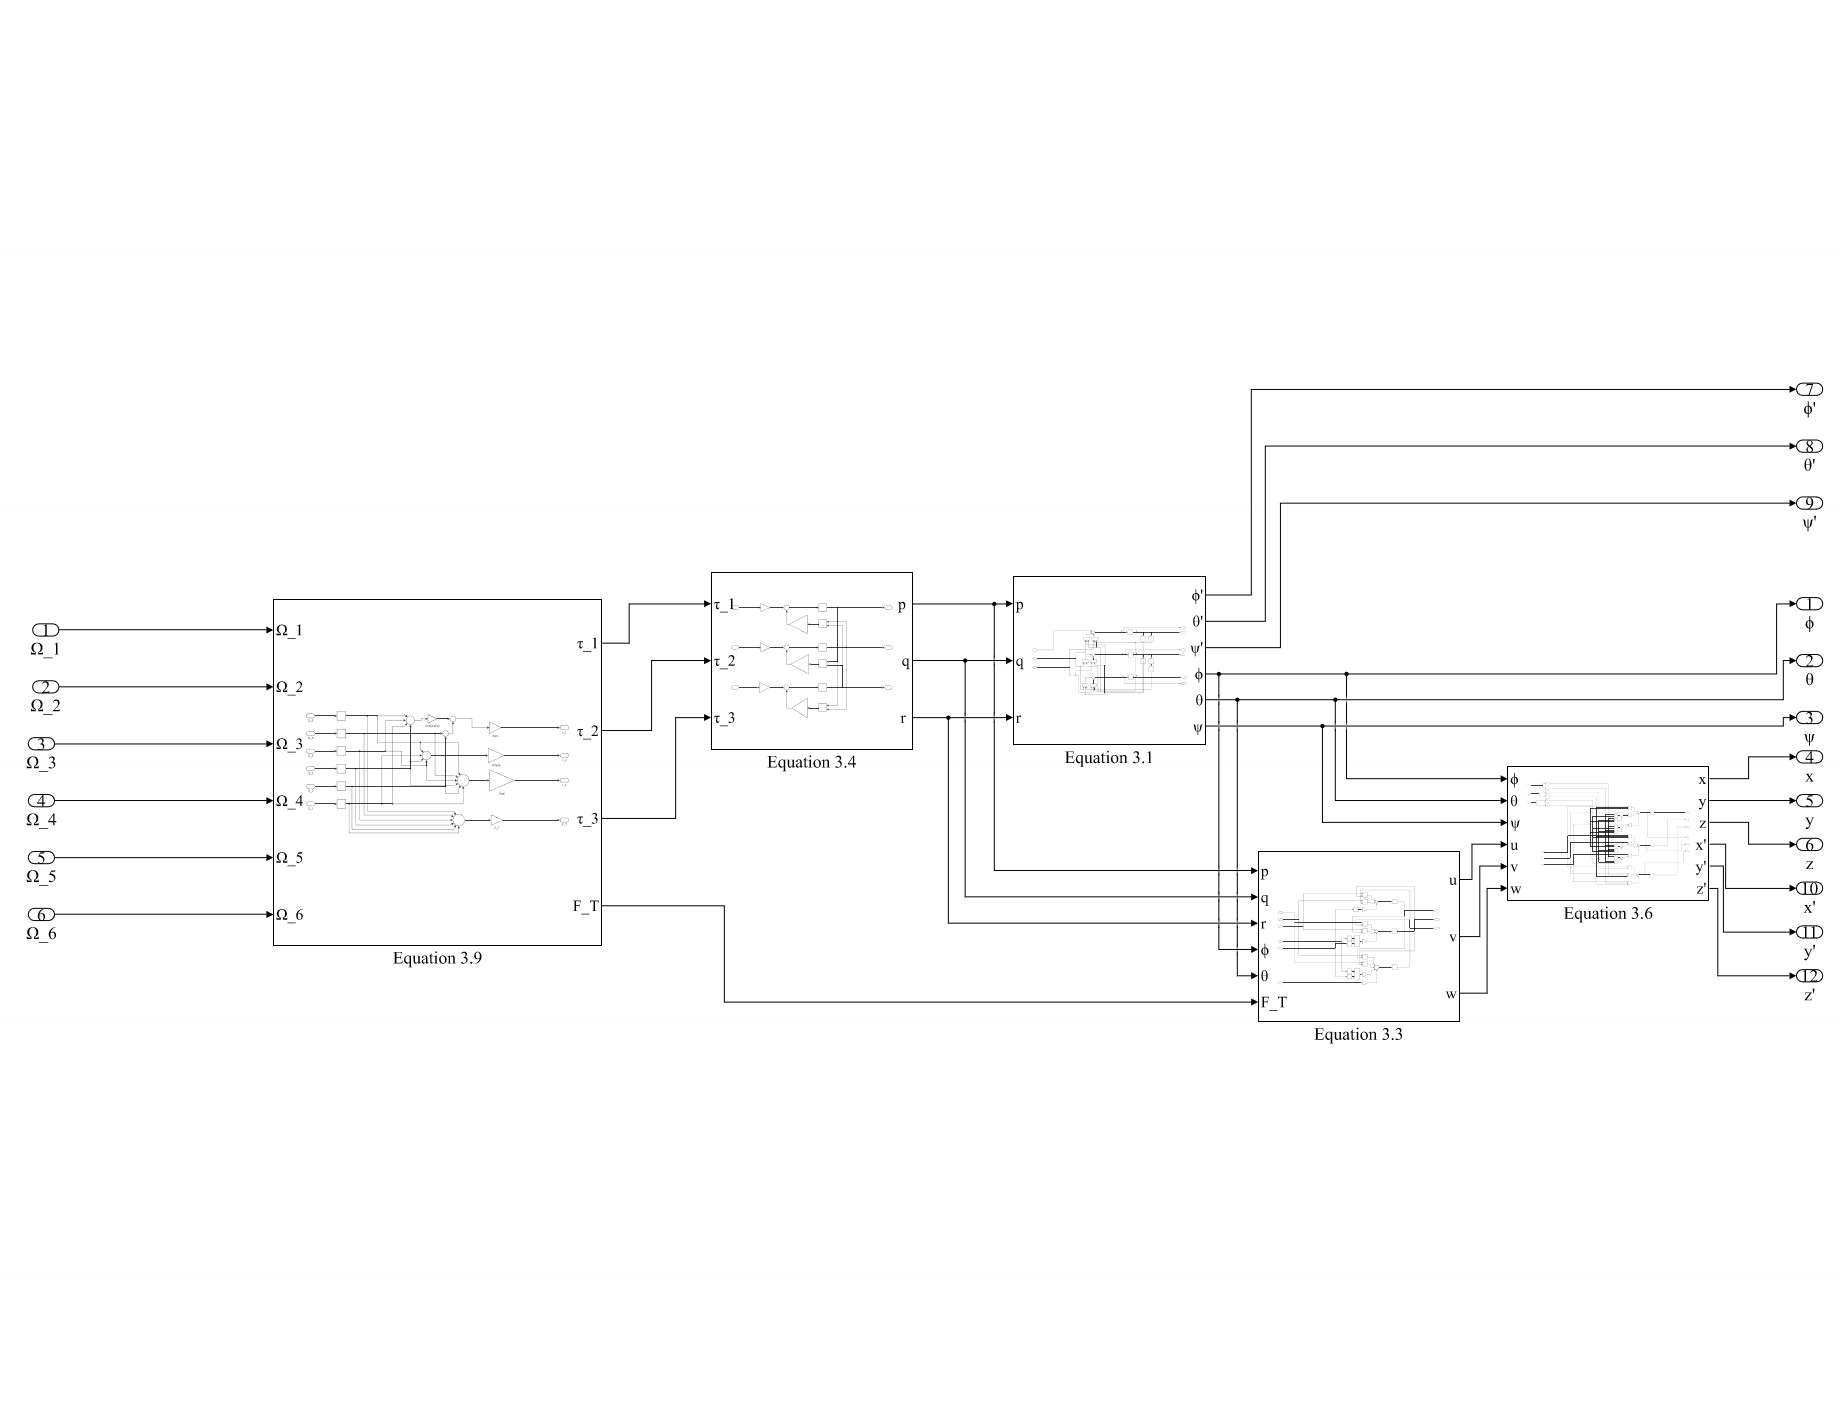
\includegraphics[width=\columnwidth]{/SimulinkModels/Plant/Plant.jpg}%
	\end{center}
	\caption{Hexacopter plant Simulink model overview.}%
\end{figure}

\begin{figure}[htb]
\begin{center}
	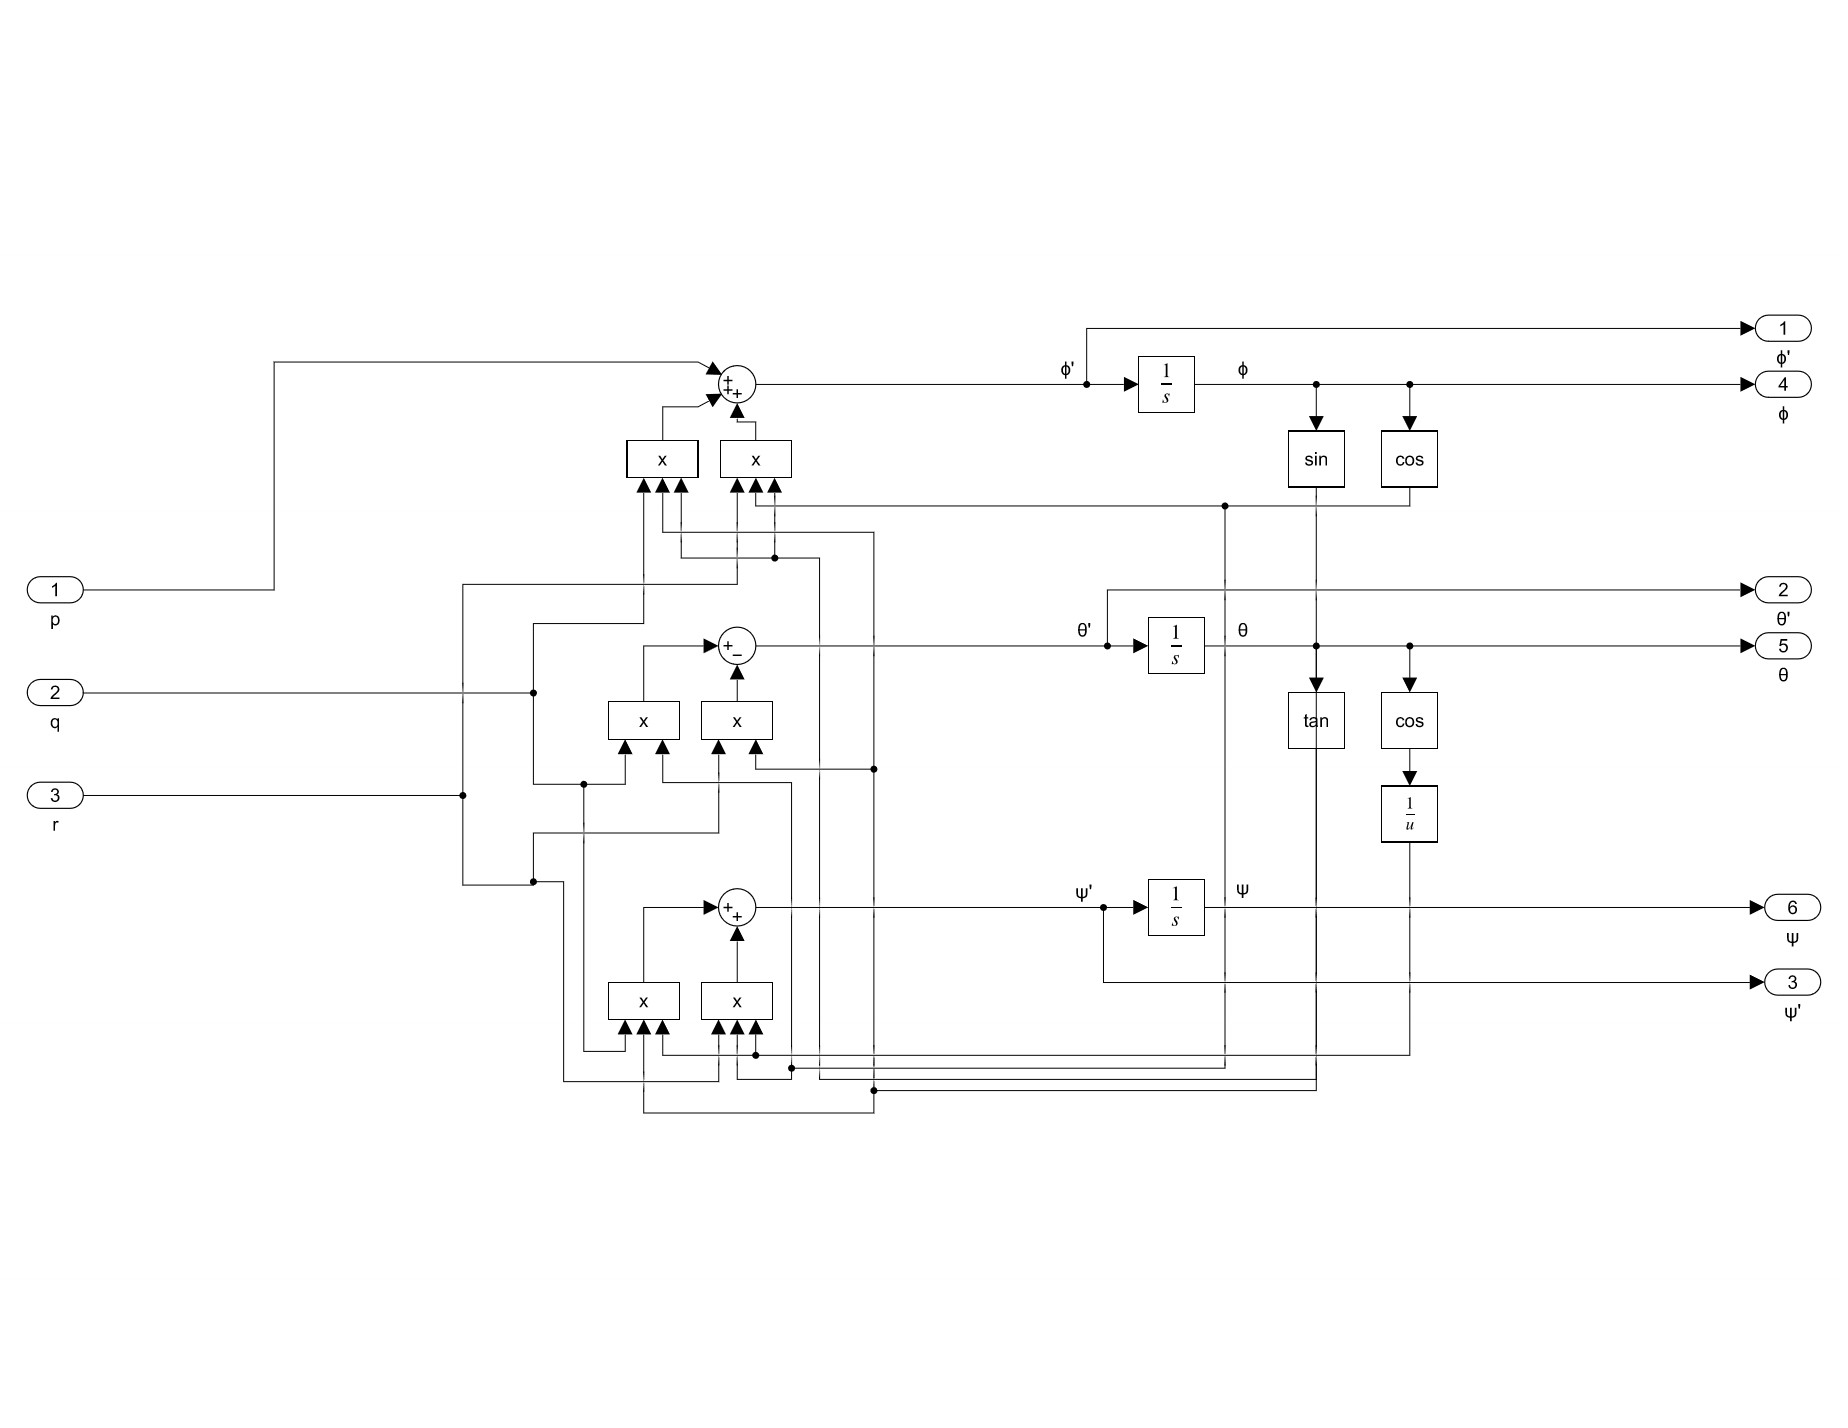
\includegraphics[width=\columnwidth]{/SimulinkModels/Plant/Eq3.1.jpg}%
	\end{center}
	\caption{Equation 3.1 Simulink subsystem.}%
\end{figure}

\begin{figure}[htb]
\begin{center}
	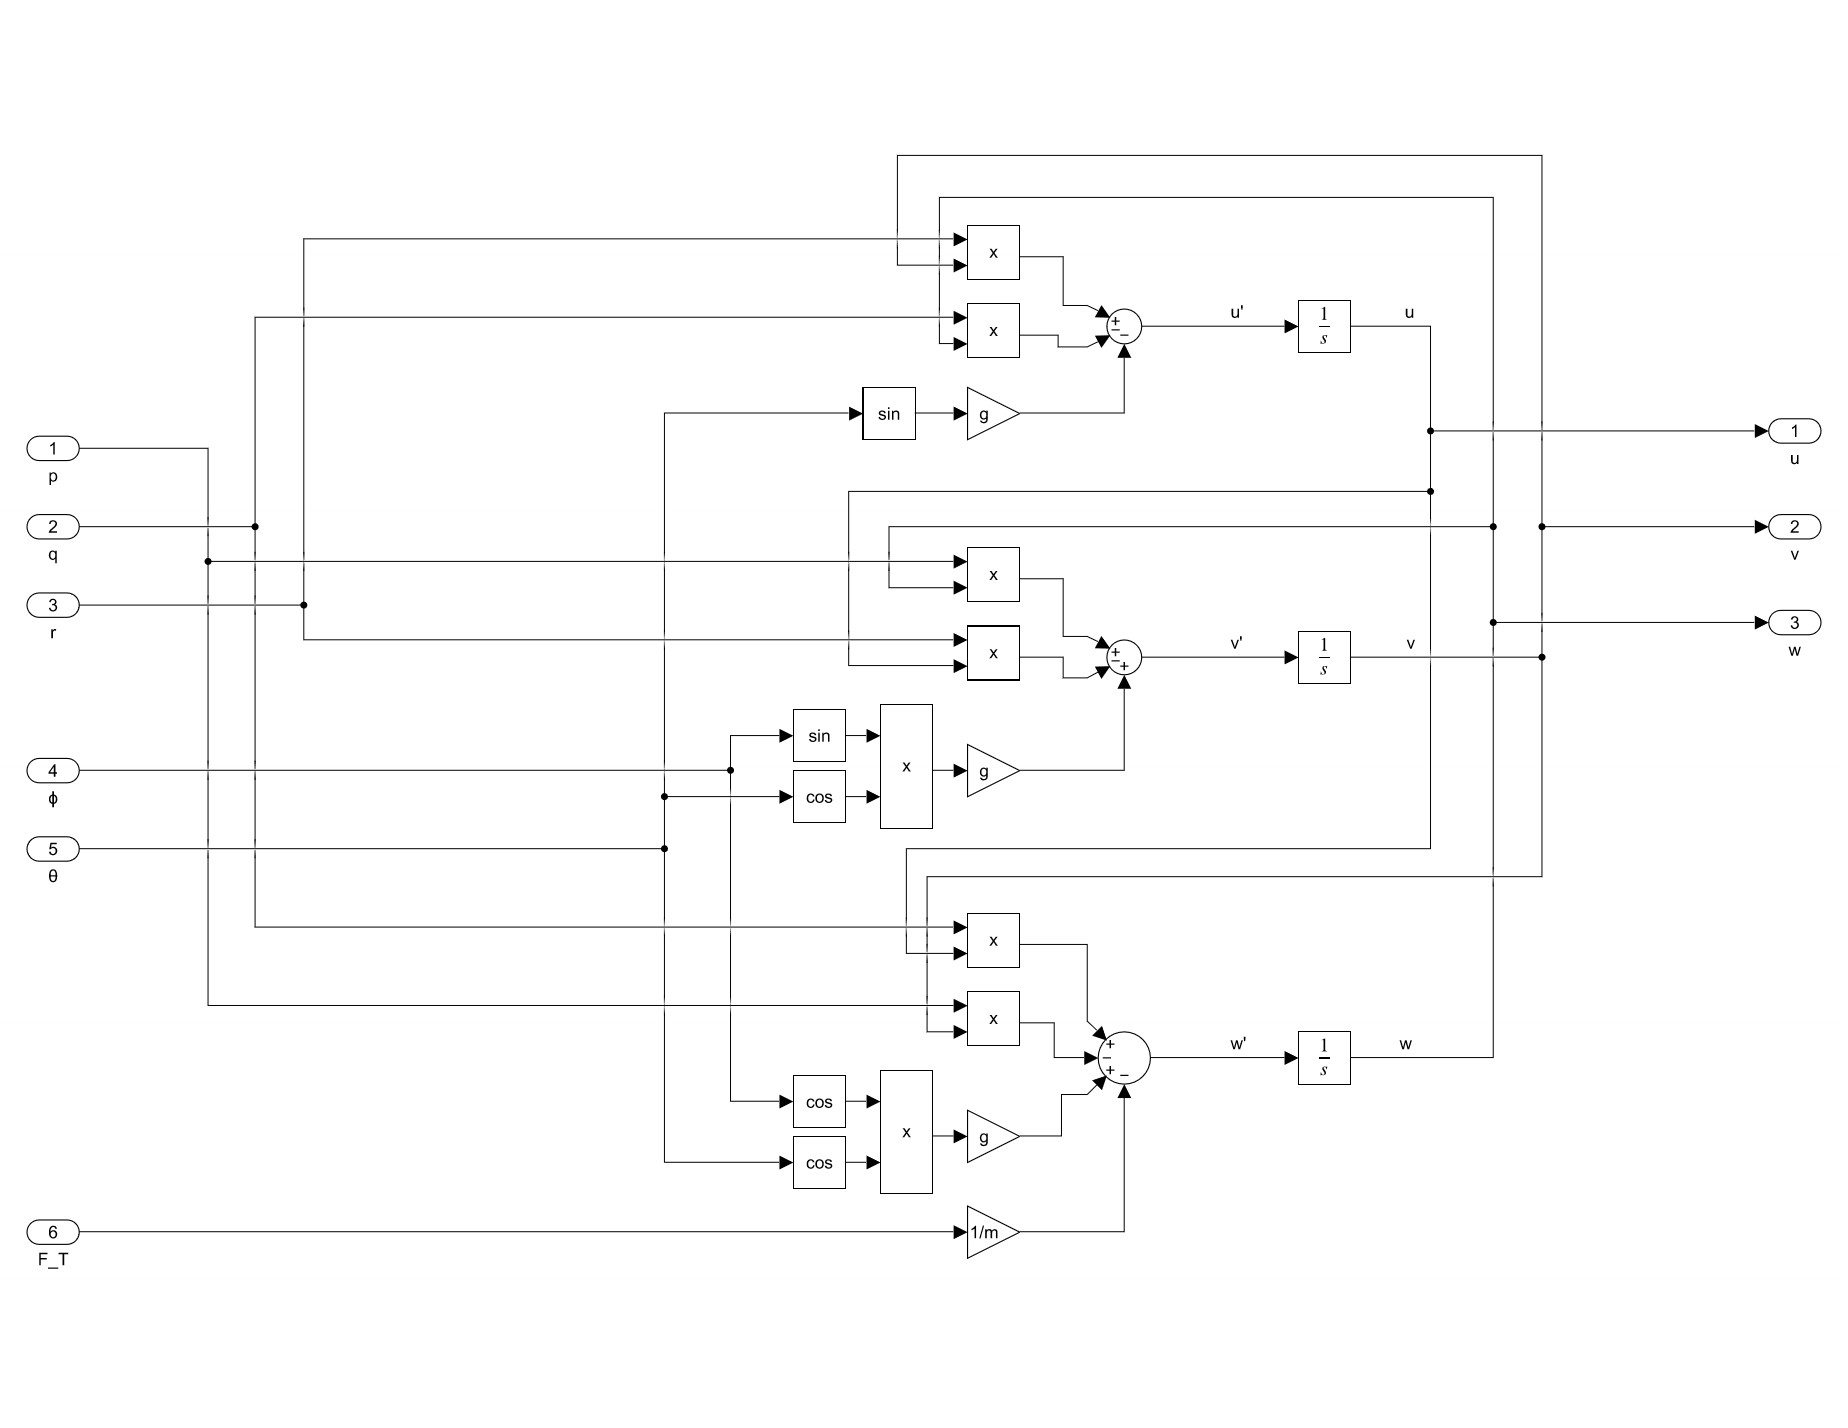
\includegraphics[width=\columnwidth]{/SimulinkModels/Plant/Eq3.3.jpg}%
	\end{center}
	\caption{Equation 3.3 Simulink subsystem.}%
\end{figure}

\begin{figure}[htb]
\begin{center}
	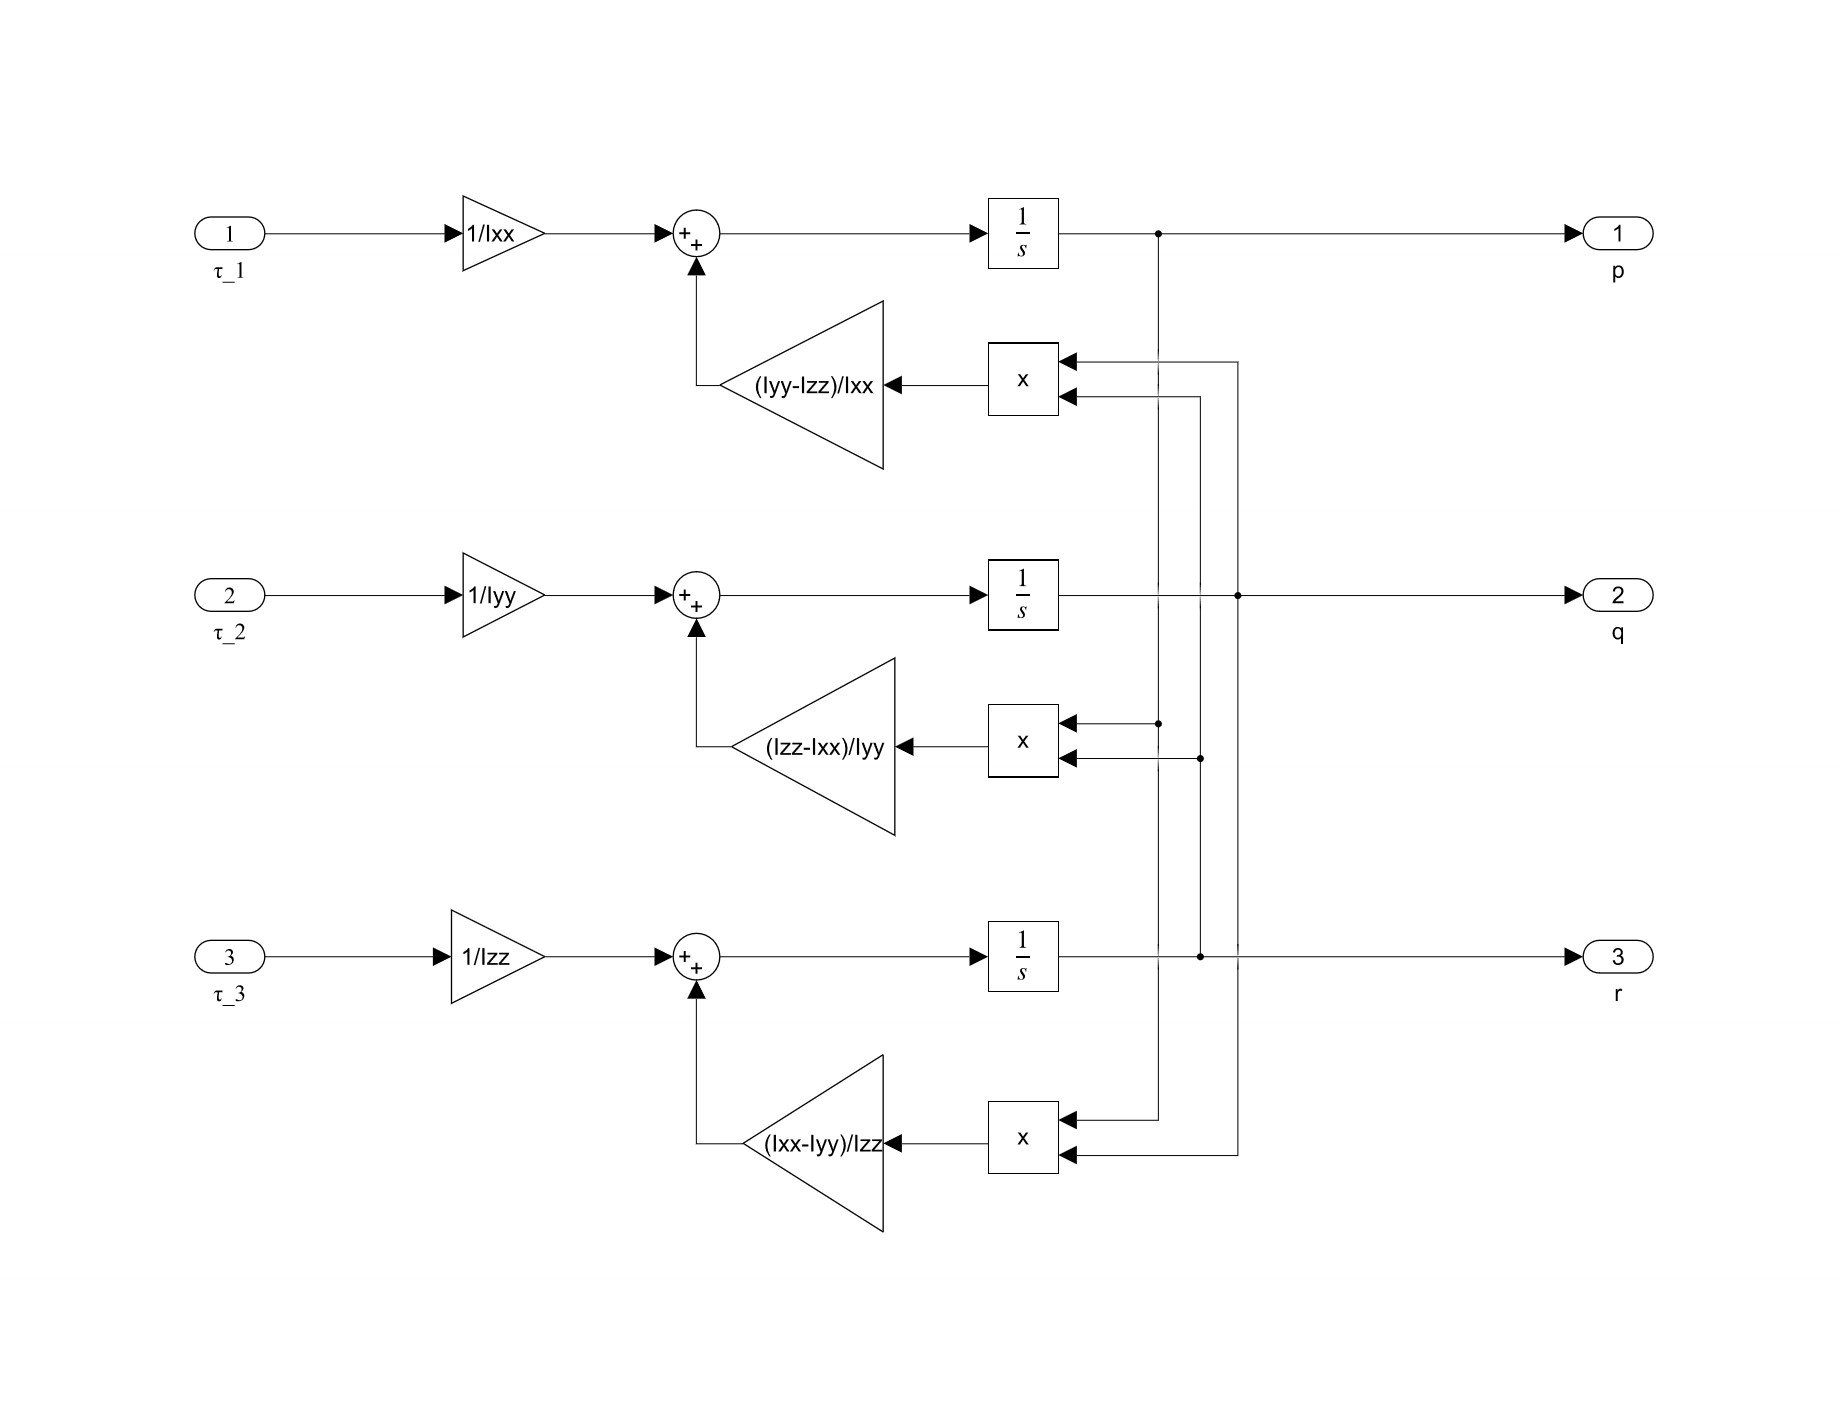
\includegraphics[width=\columnwidth]{/SimulinkModels/Plant/Eq3.4.jpg}%
	\end{center}
	\caption{Equation 3.4 Simulink subsystem.}%
\end{figure}

\begin{figure}[htb]
\begin{center}
	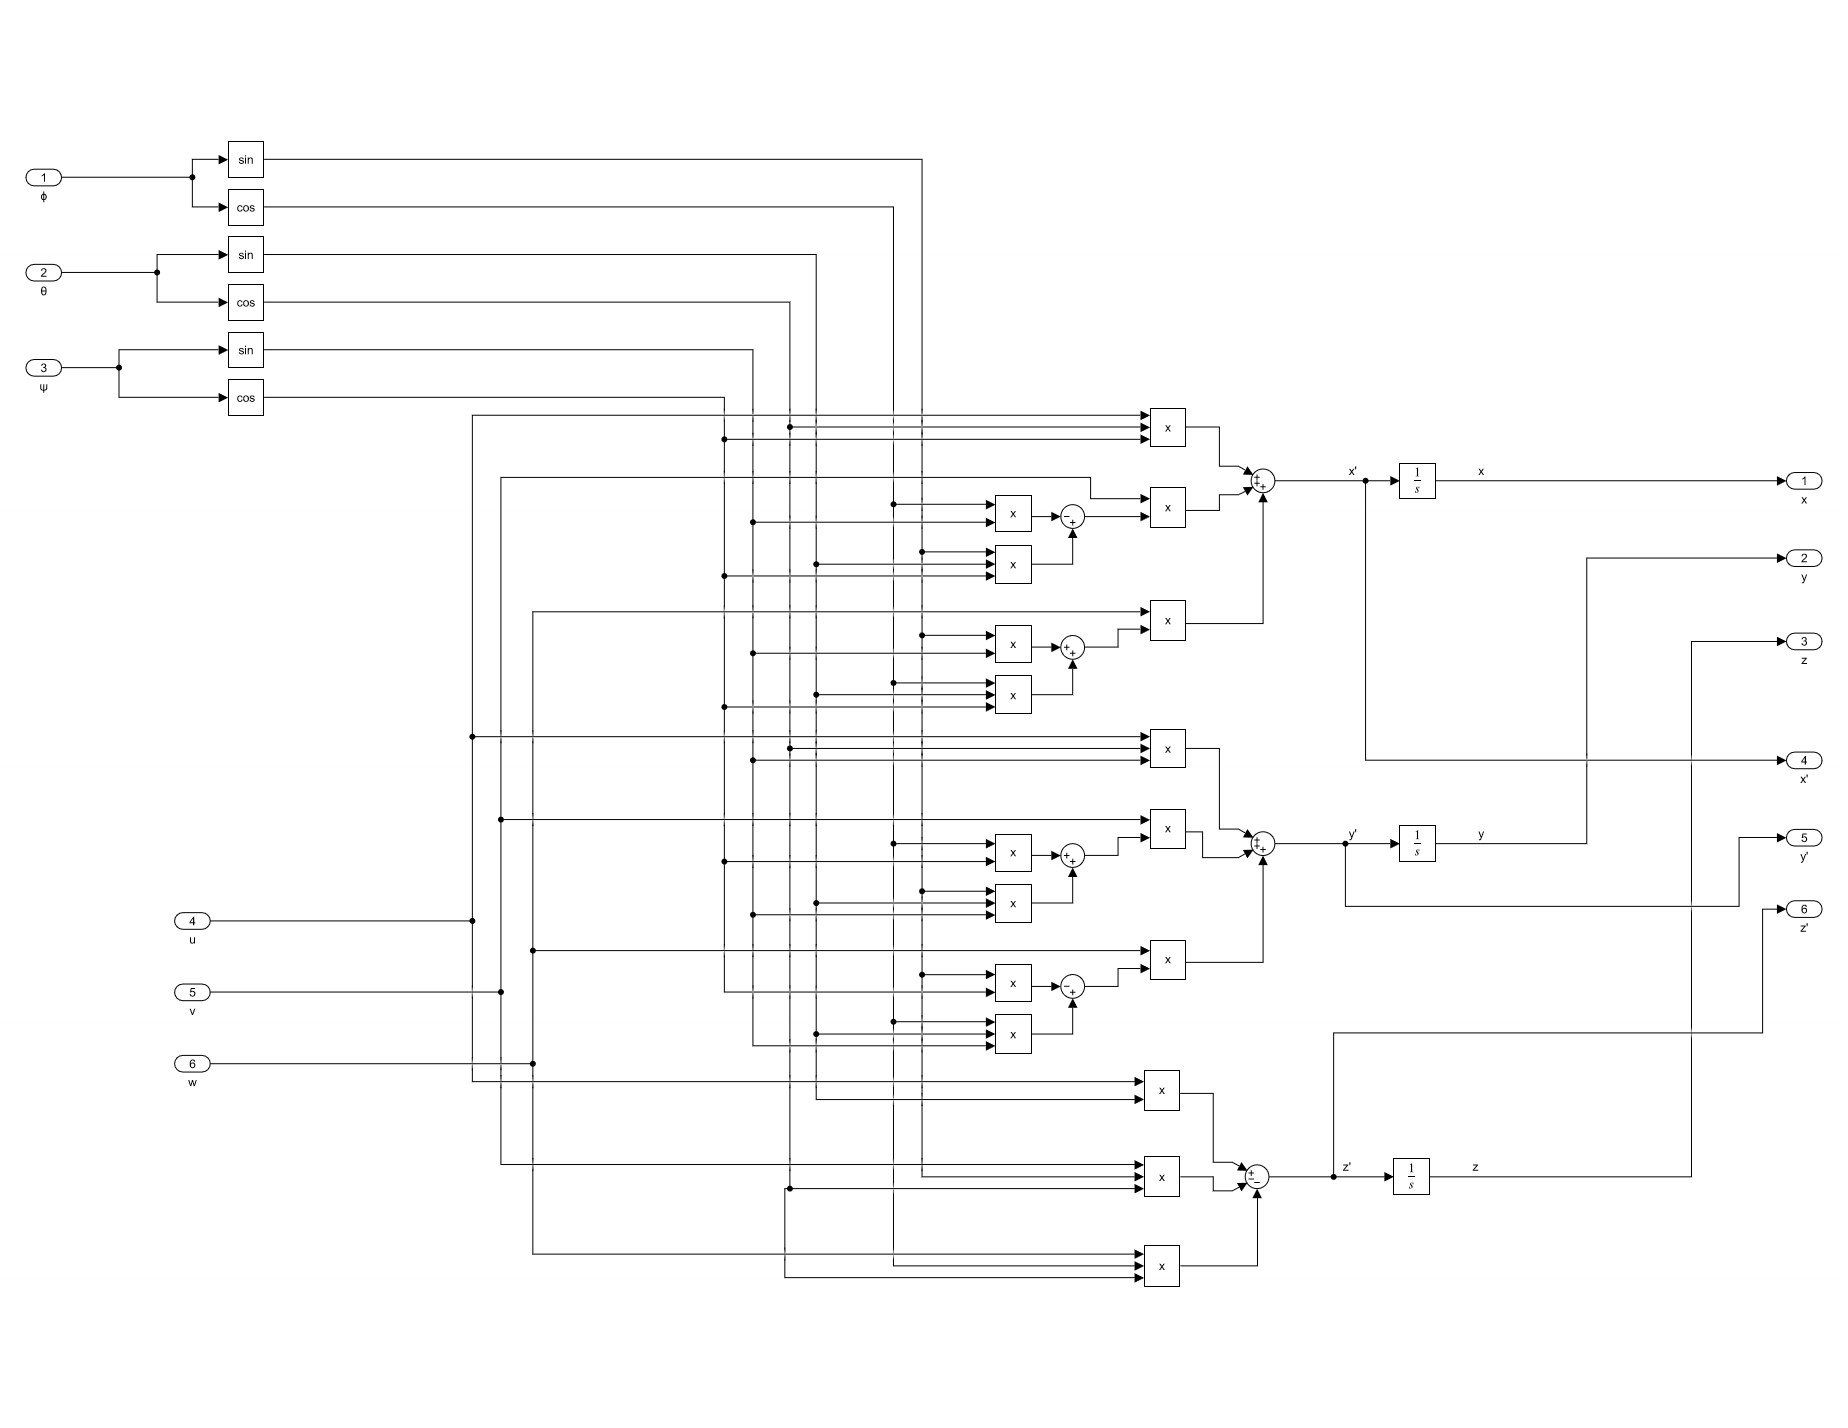
\includegraphics[width=\columnwidth]{/SimulinkModels/Plant/Eq3.6.jpg}%
	\end{center}
	\caption{Equation 3.6 Simulink subsystem.}%	
\end{figure}

\begin{figure}[htb]
\begin{center}
	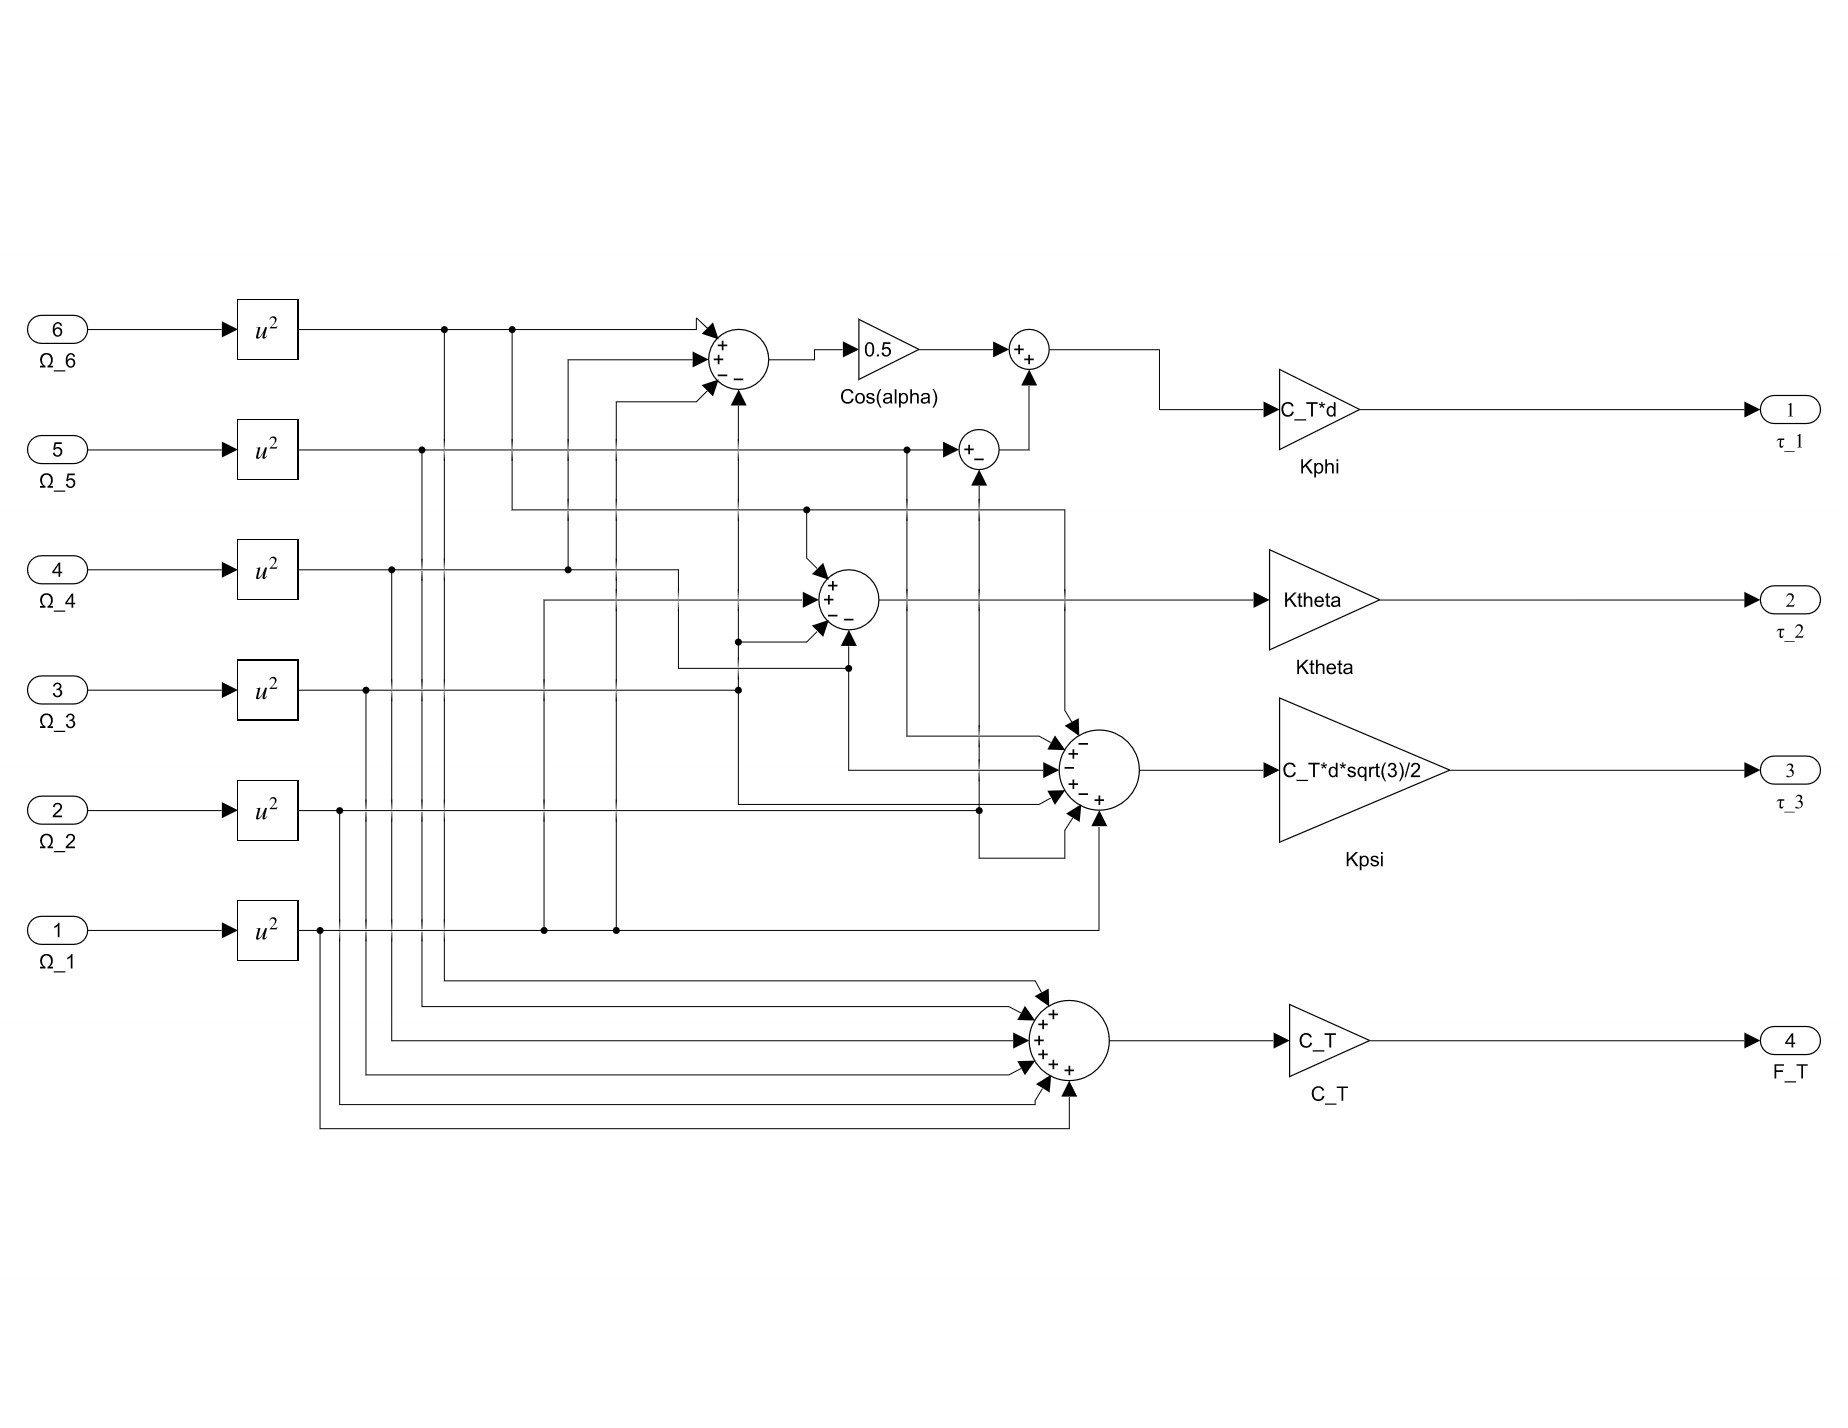
\includegraphics[width=\columnwidth]{/SimulinkModels/Plant/Eq3.9.jpg}%
	\end{center}
	\caption{Equation 3.9 Simulink subsystem.}%	
\end{figure}


\FloatBarrier
\clearpage
\section{Control Inputs to Motor Speeds}

\begin{figure}[htb]
\begin{center}
	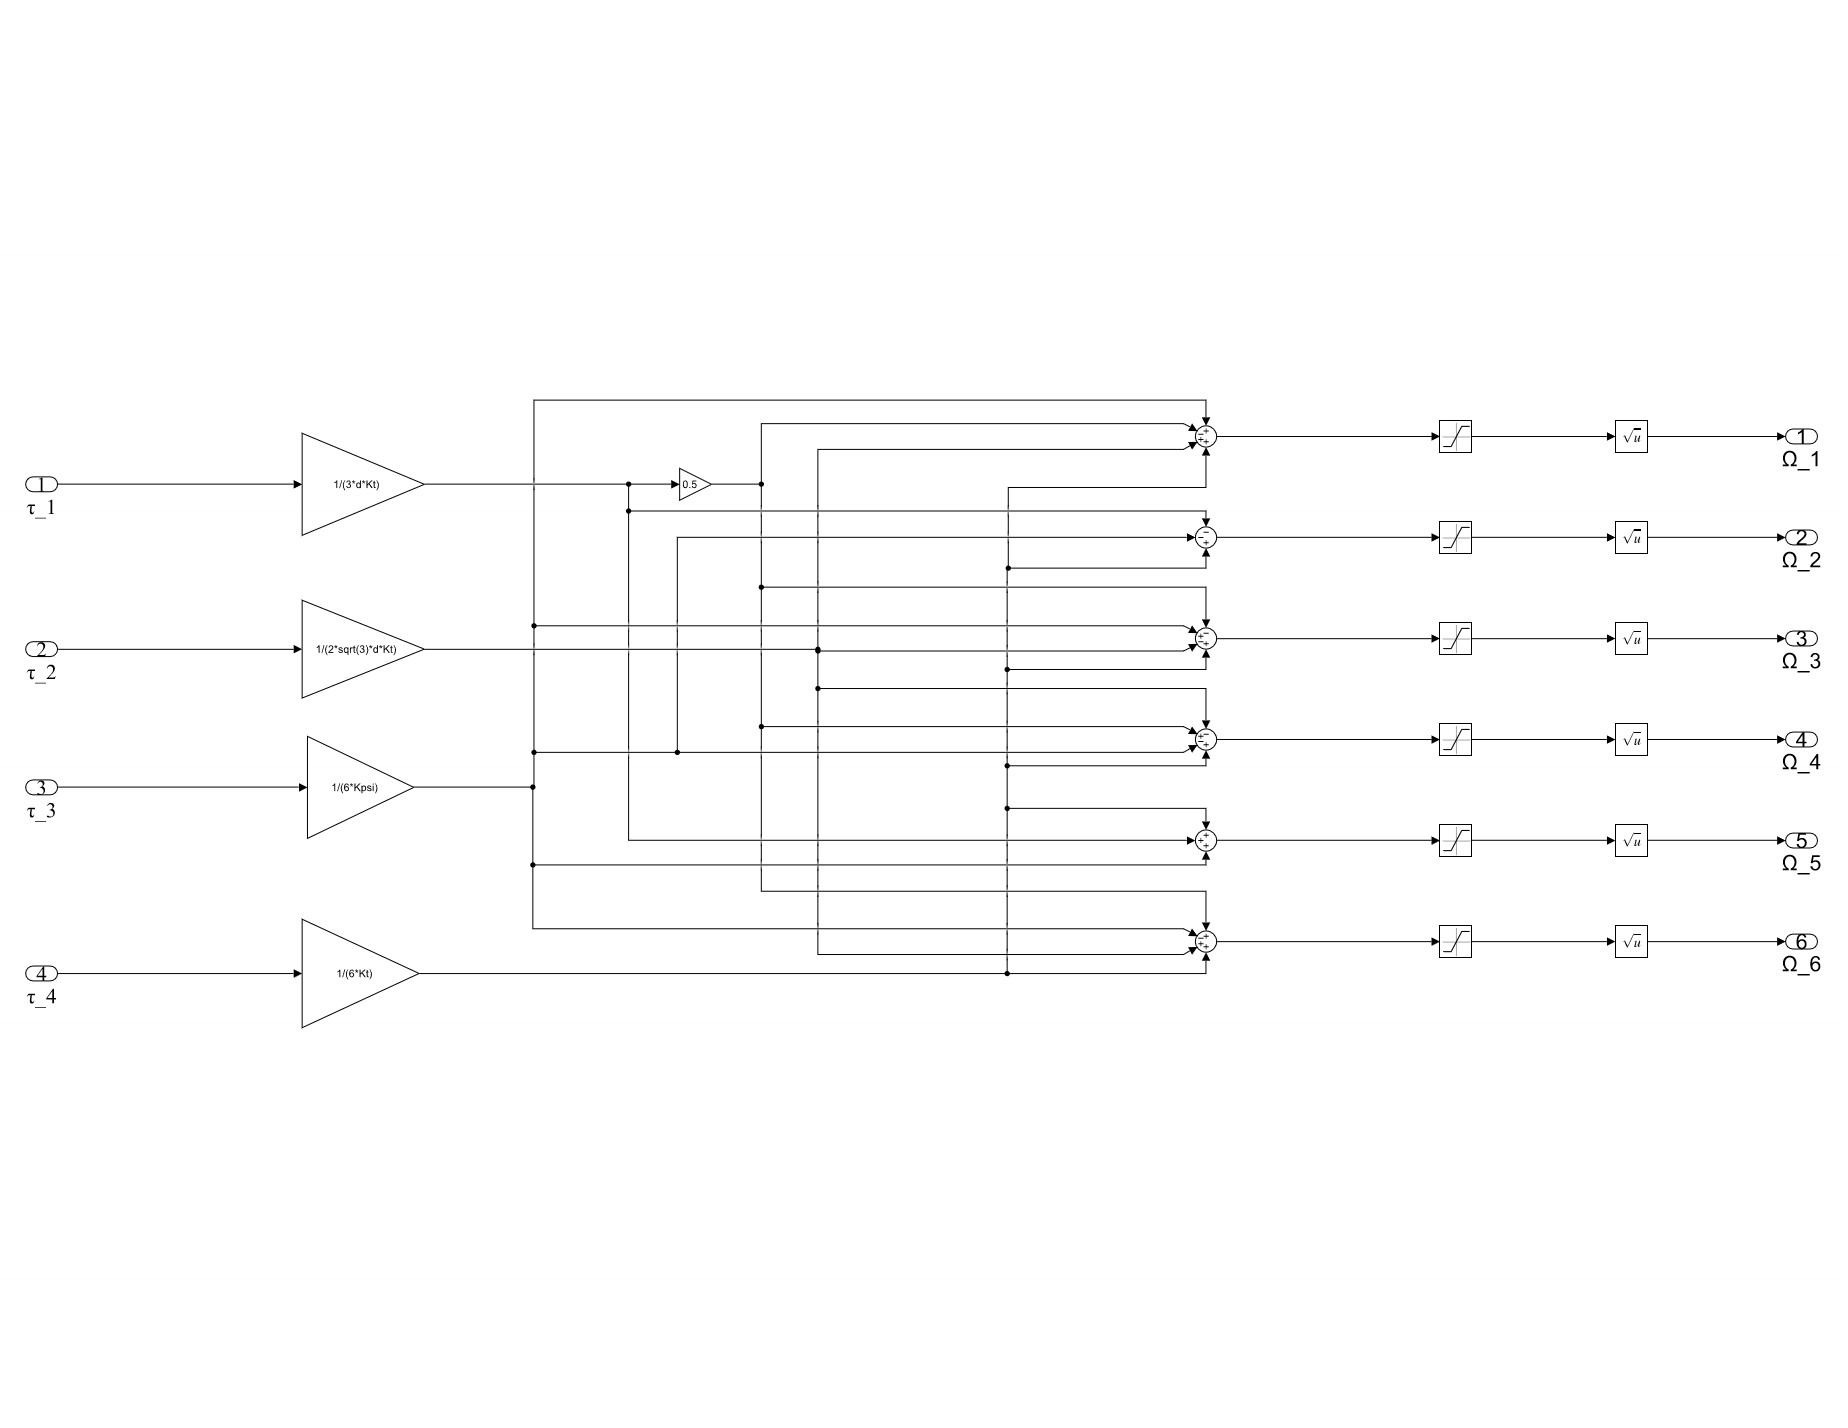
\includegraphics[width=\columnwidth]{/SimulinkModels/InputsToSpeeds.jpg}%
	\end{center}
	\caption{Equation 3.9 Simulink subsystem.}%	
\end{figure}
\FloatBarrier
\clearpage

\section{Control System}

\begin{figure}[htb]
\begin{center}
	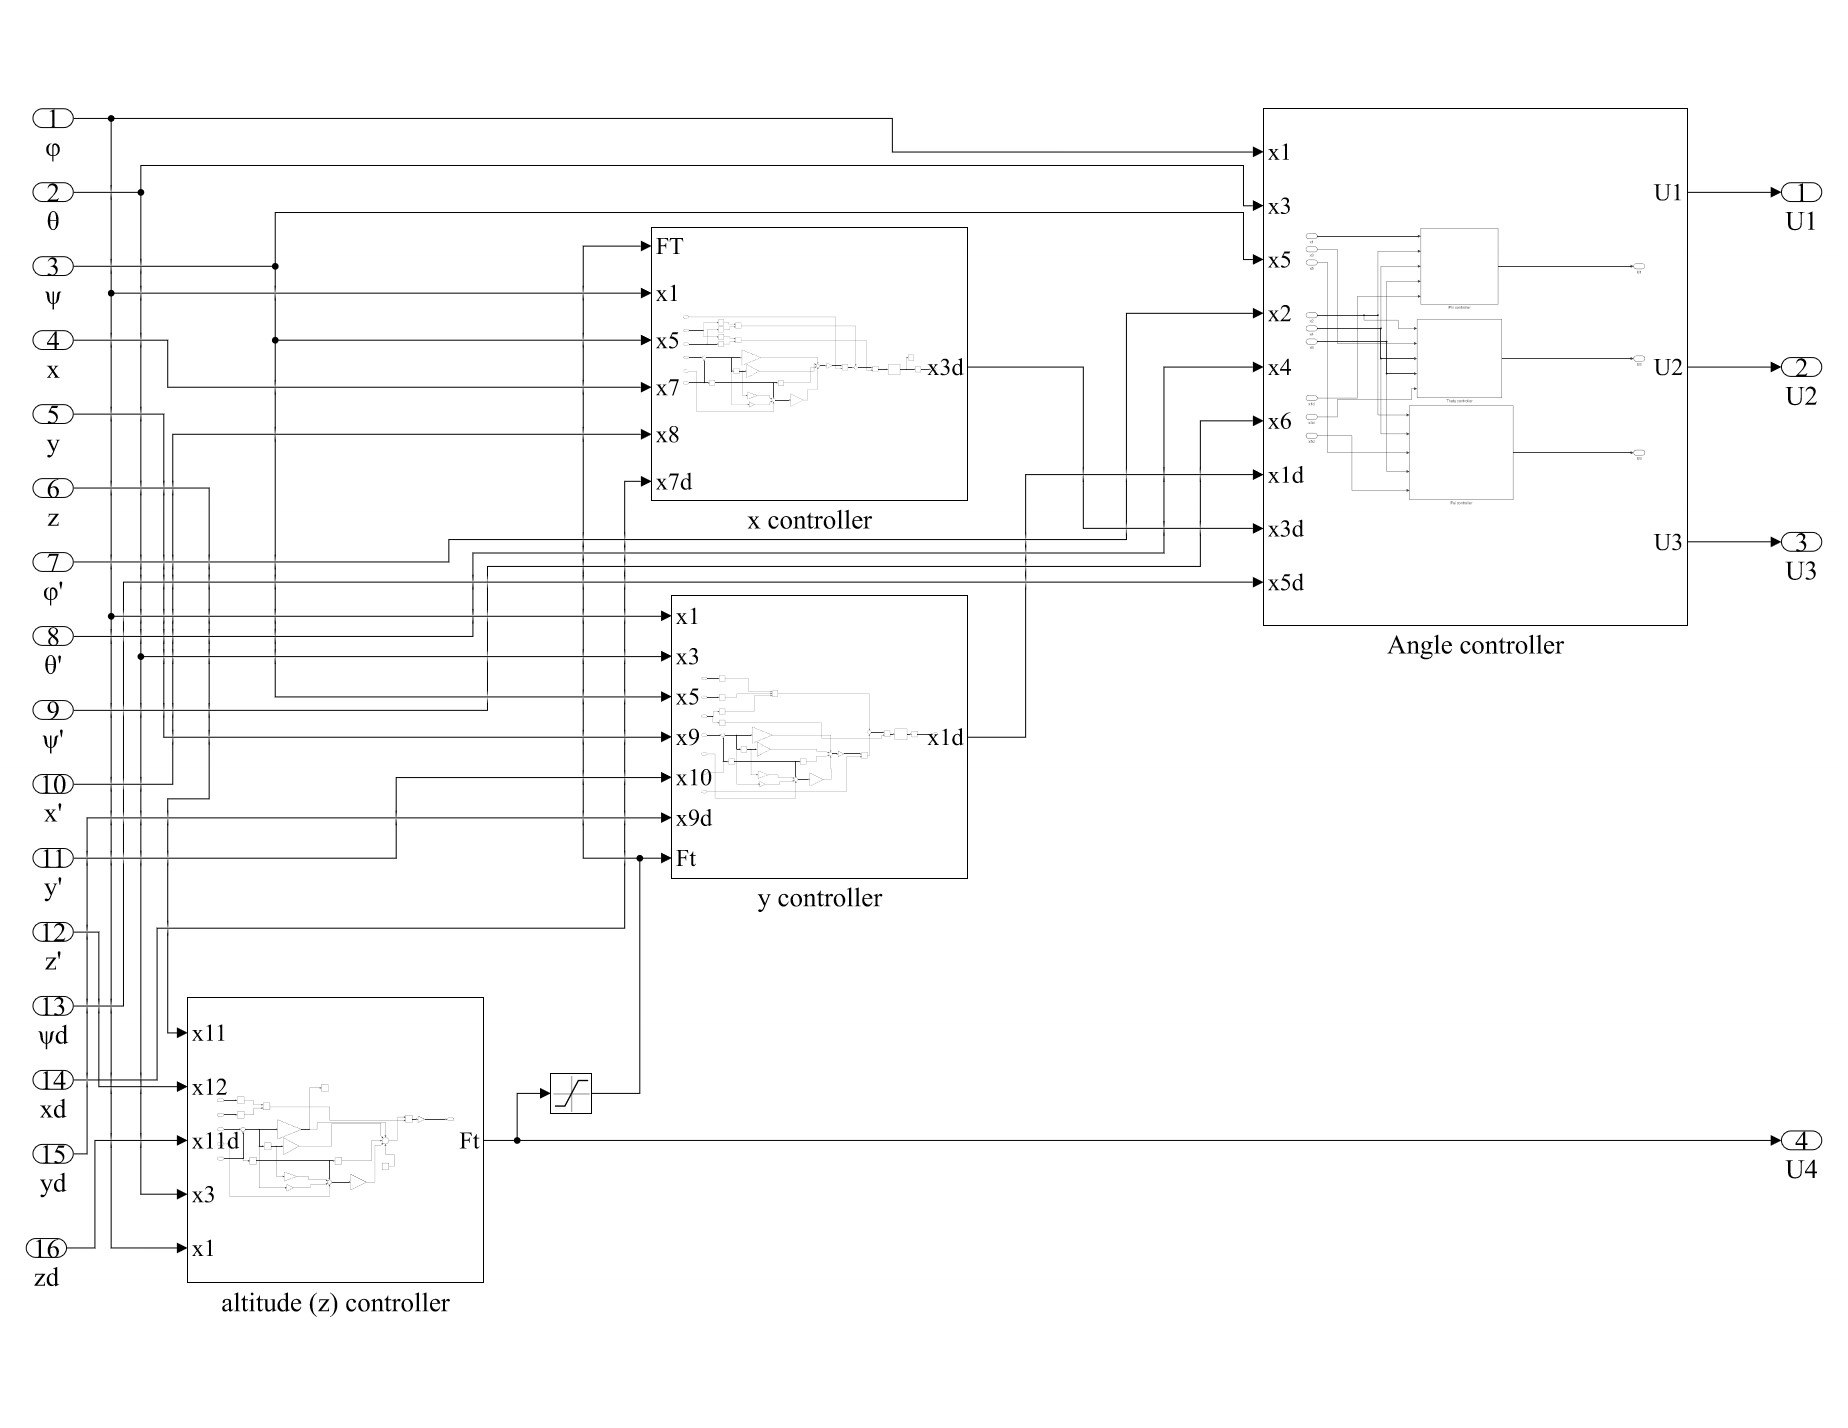
\includegraphics[width=\columnwidth]{/SimulinkModels/Controller/Controller.jpg}%
	\end{center}
	\caption{Control system Simulink model overview.}%
\end{figure}

\begin{figure}[htb]
\begin{center}
	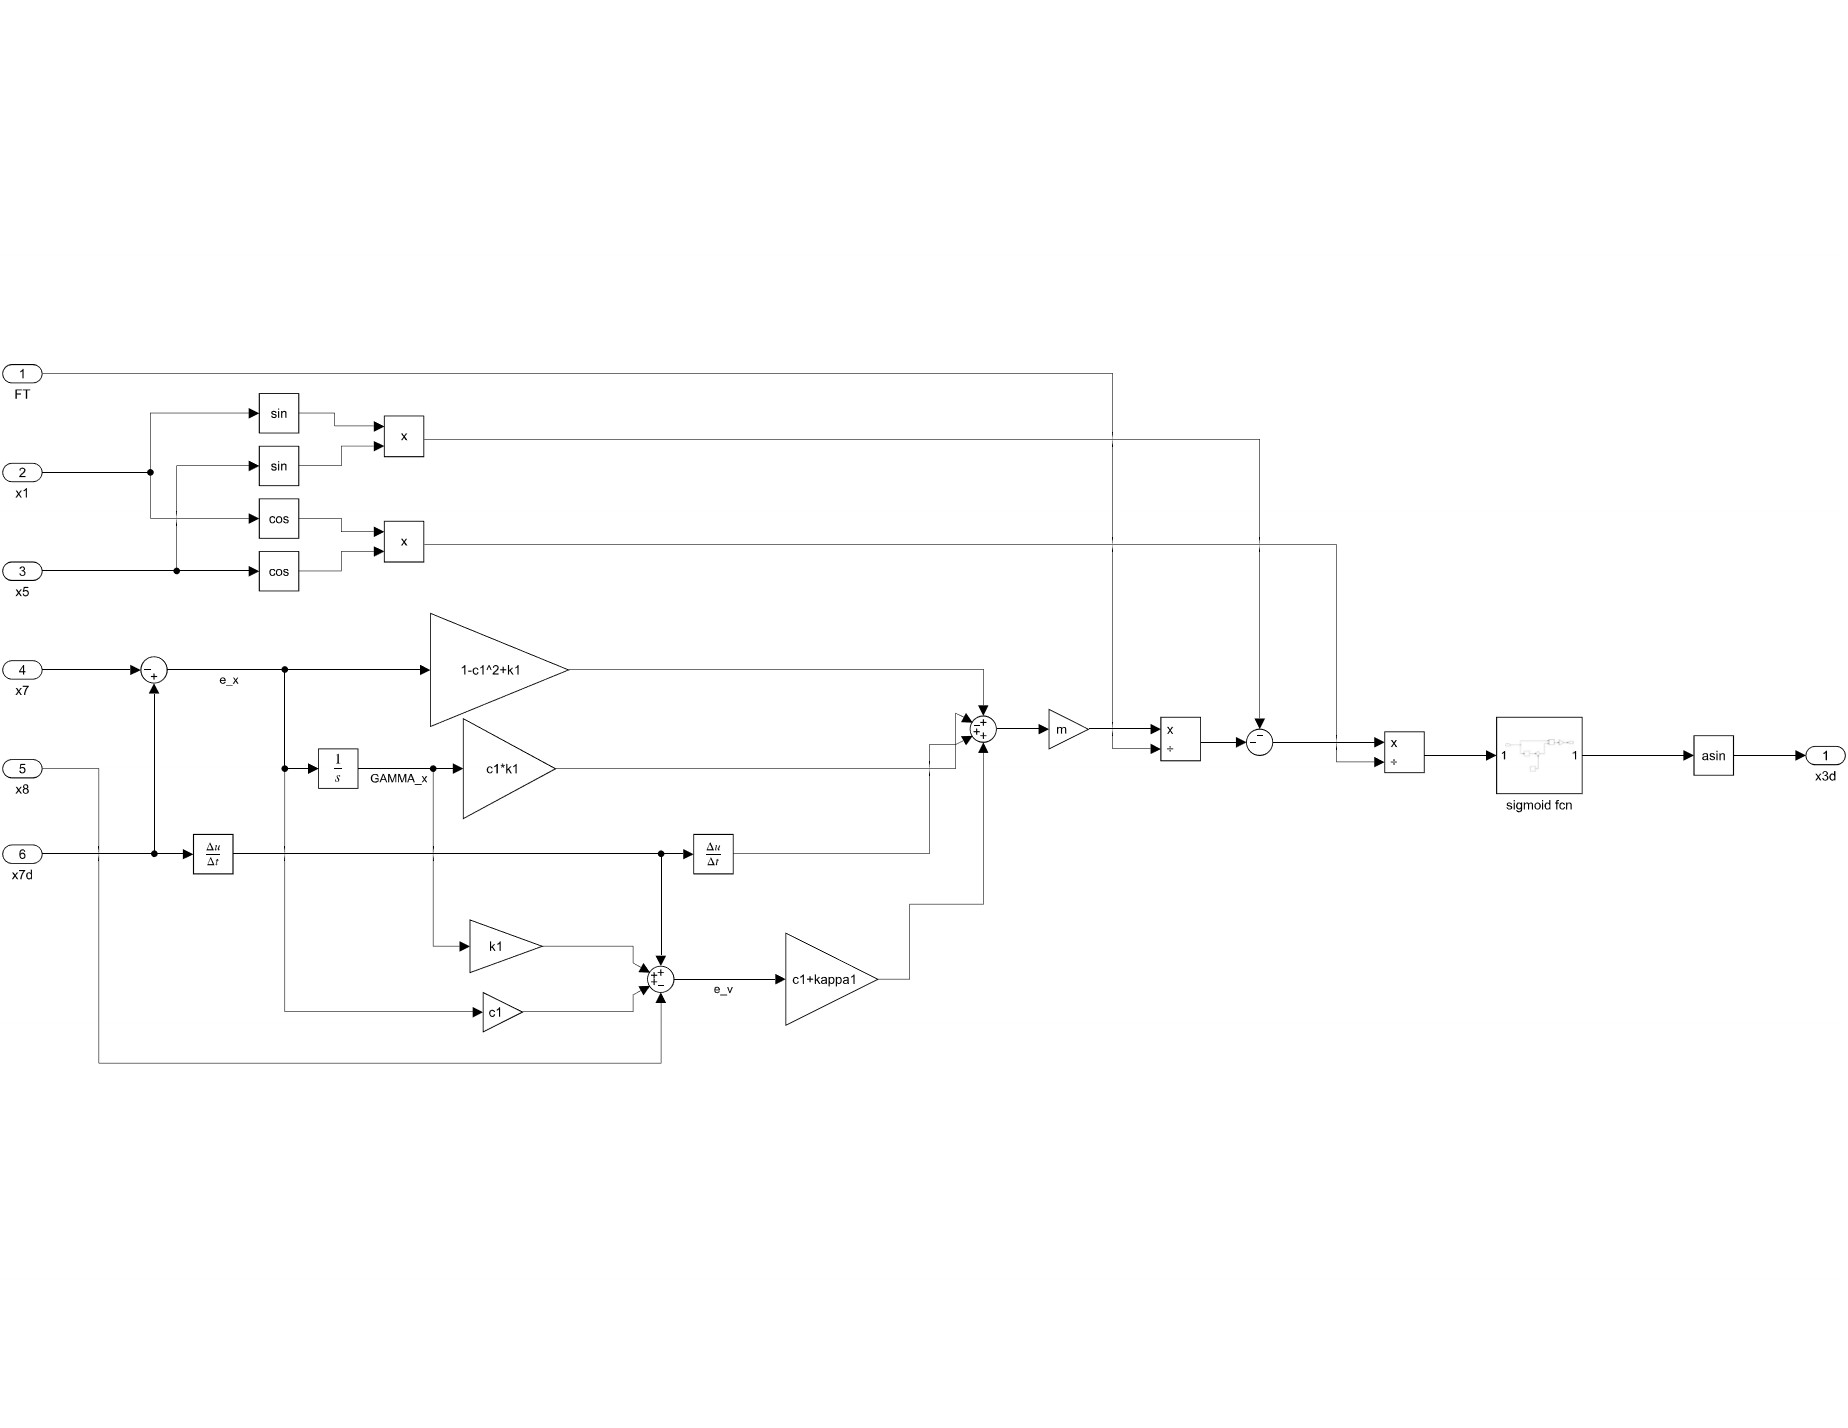
\includegraphics[width=\columnwidth]{/SimulinkModels/Controller/x.jpg}%
	\end{center}
	\caption{X position controller Simulink subsystem.}%
\end{figure}

\begin{figure}[htb]
\begin{center}
	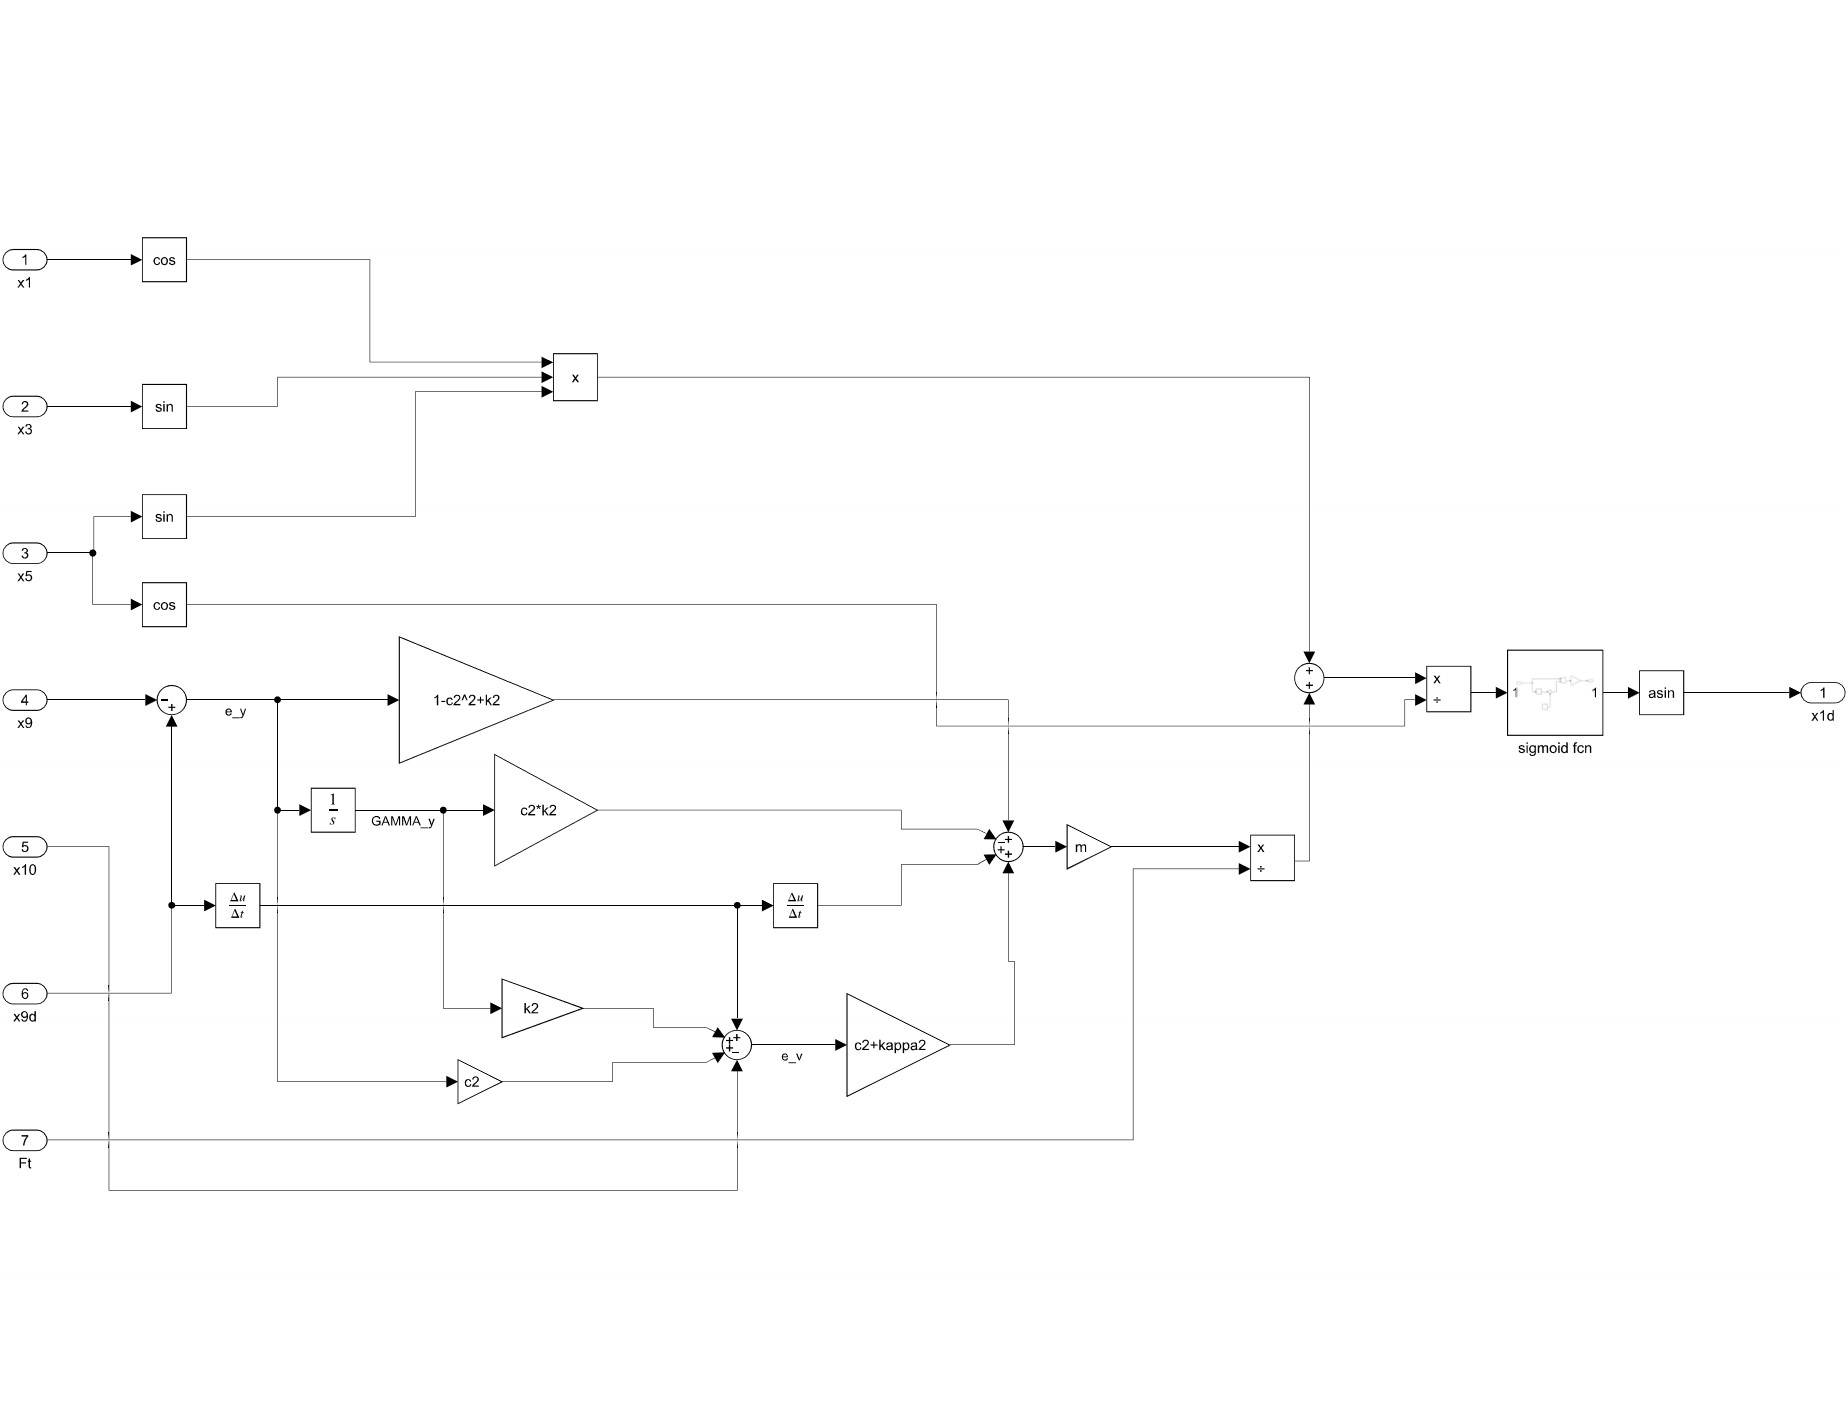
\includegraphics[width=\columnwidth]{/SimulinkModels/Controller/y.jpg}%
	\end{center}
	\caption{Y position controller Simulink subsystem.}%
\end{figure}

\begin{figure}[htb]
\begin{center}
	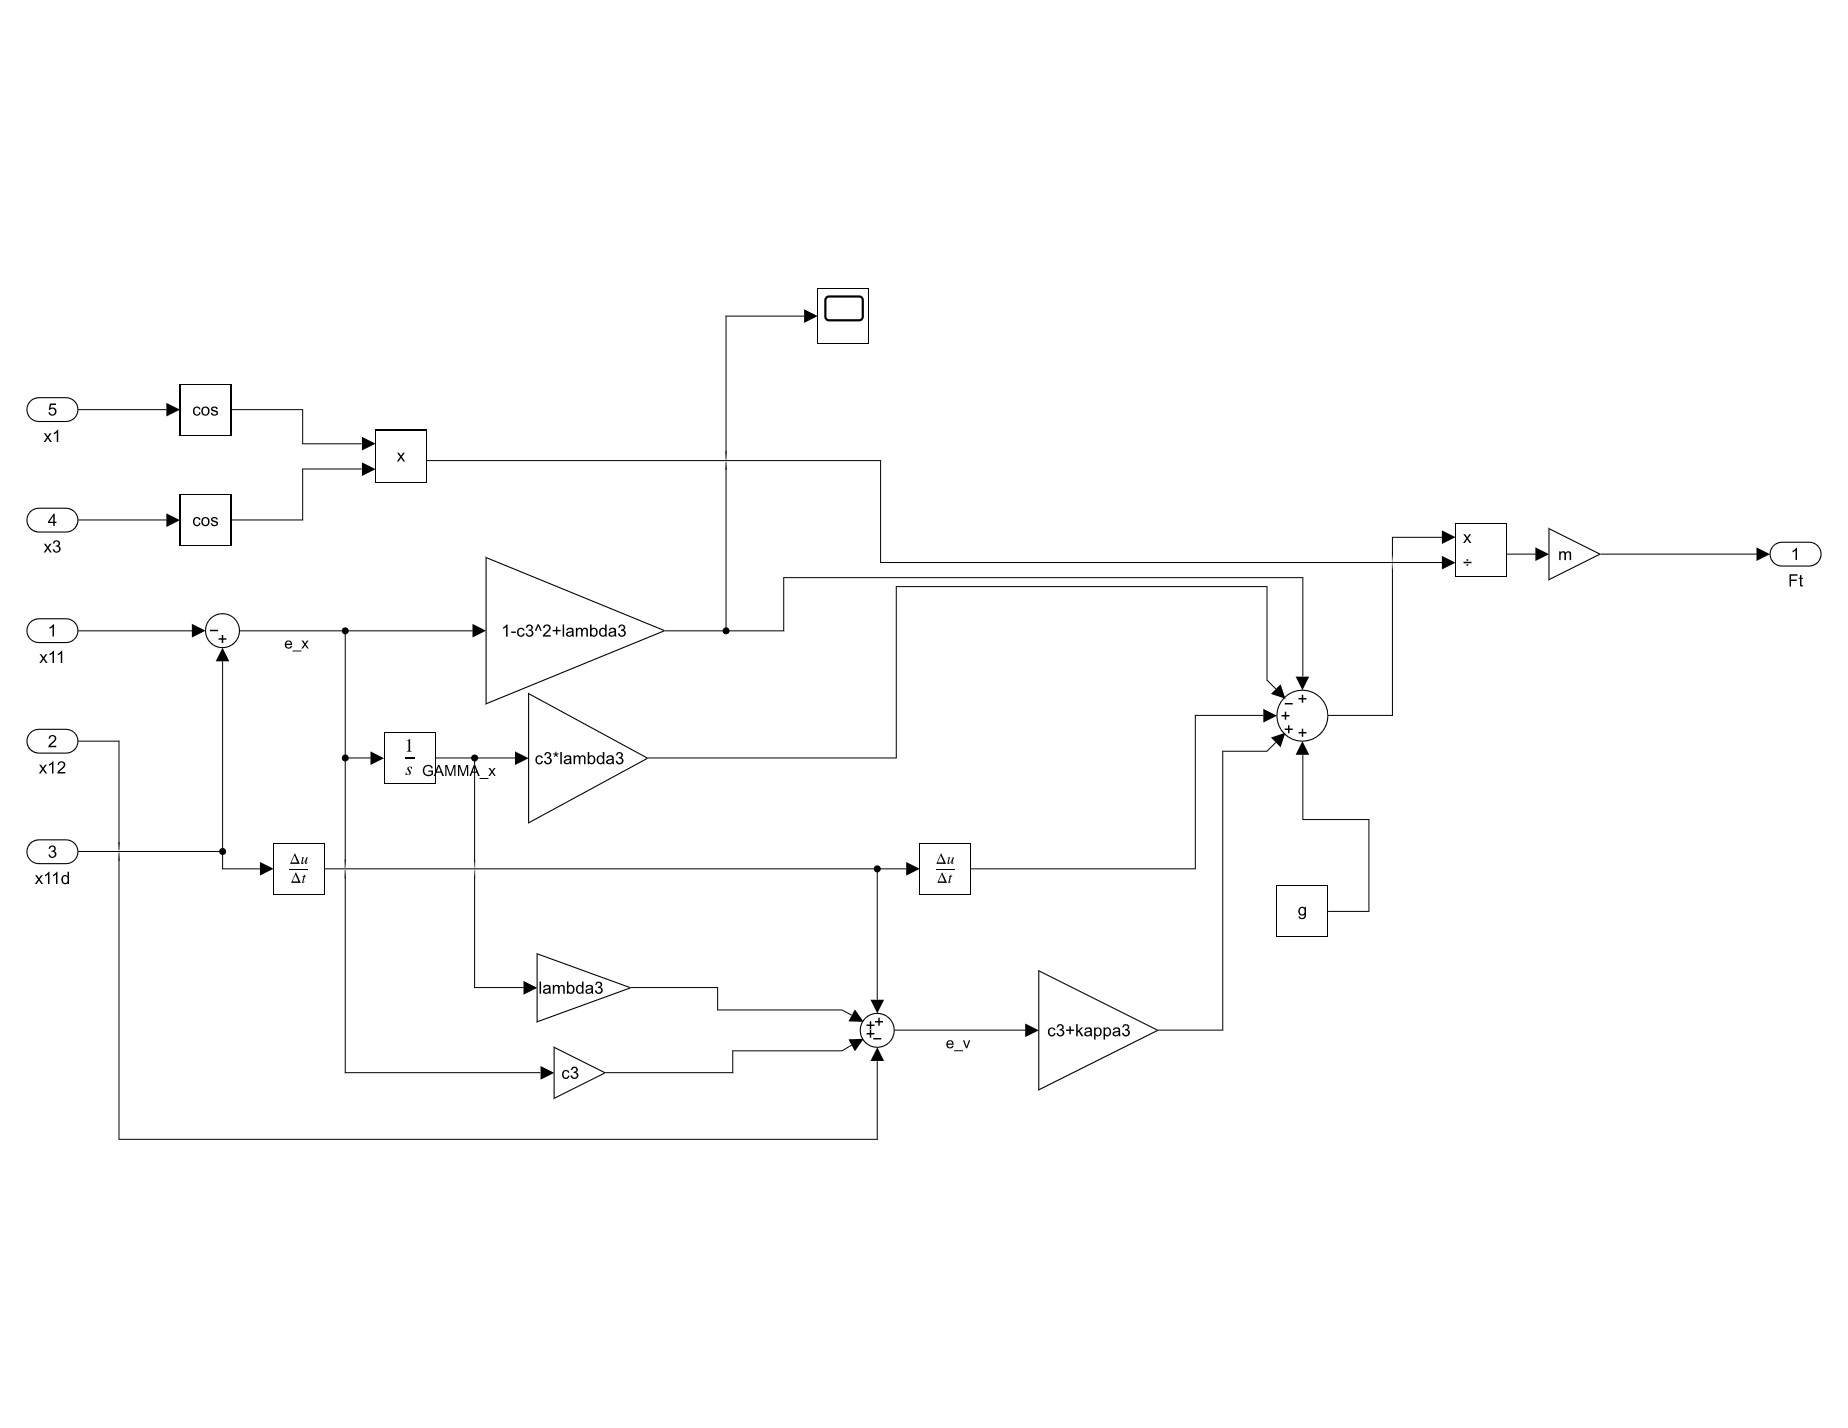
\includegraphics[width=\columnwidth]{/SimulinkModels/Controller/z.jpg}%
	\end{center}
	\caption{Z position controller Simulink subsystem.}%
\end{figure}

\begin{figure}[htb]
\begin{center}
	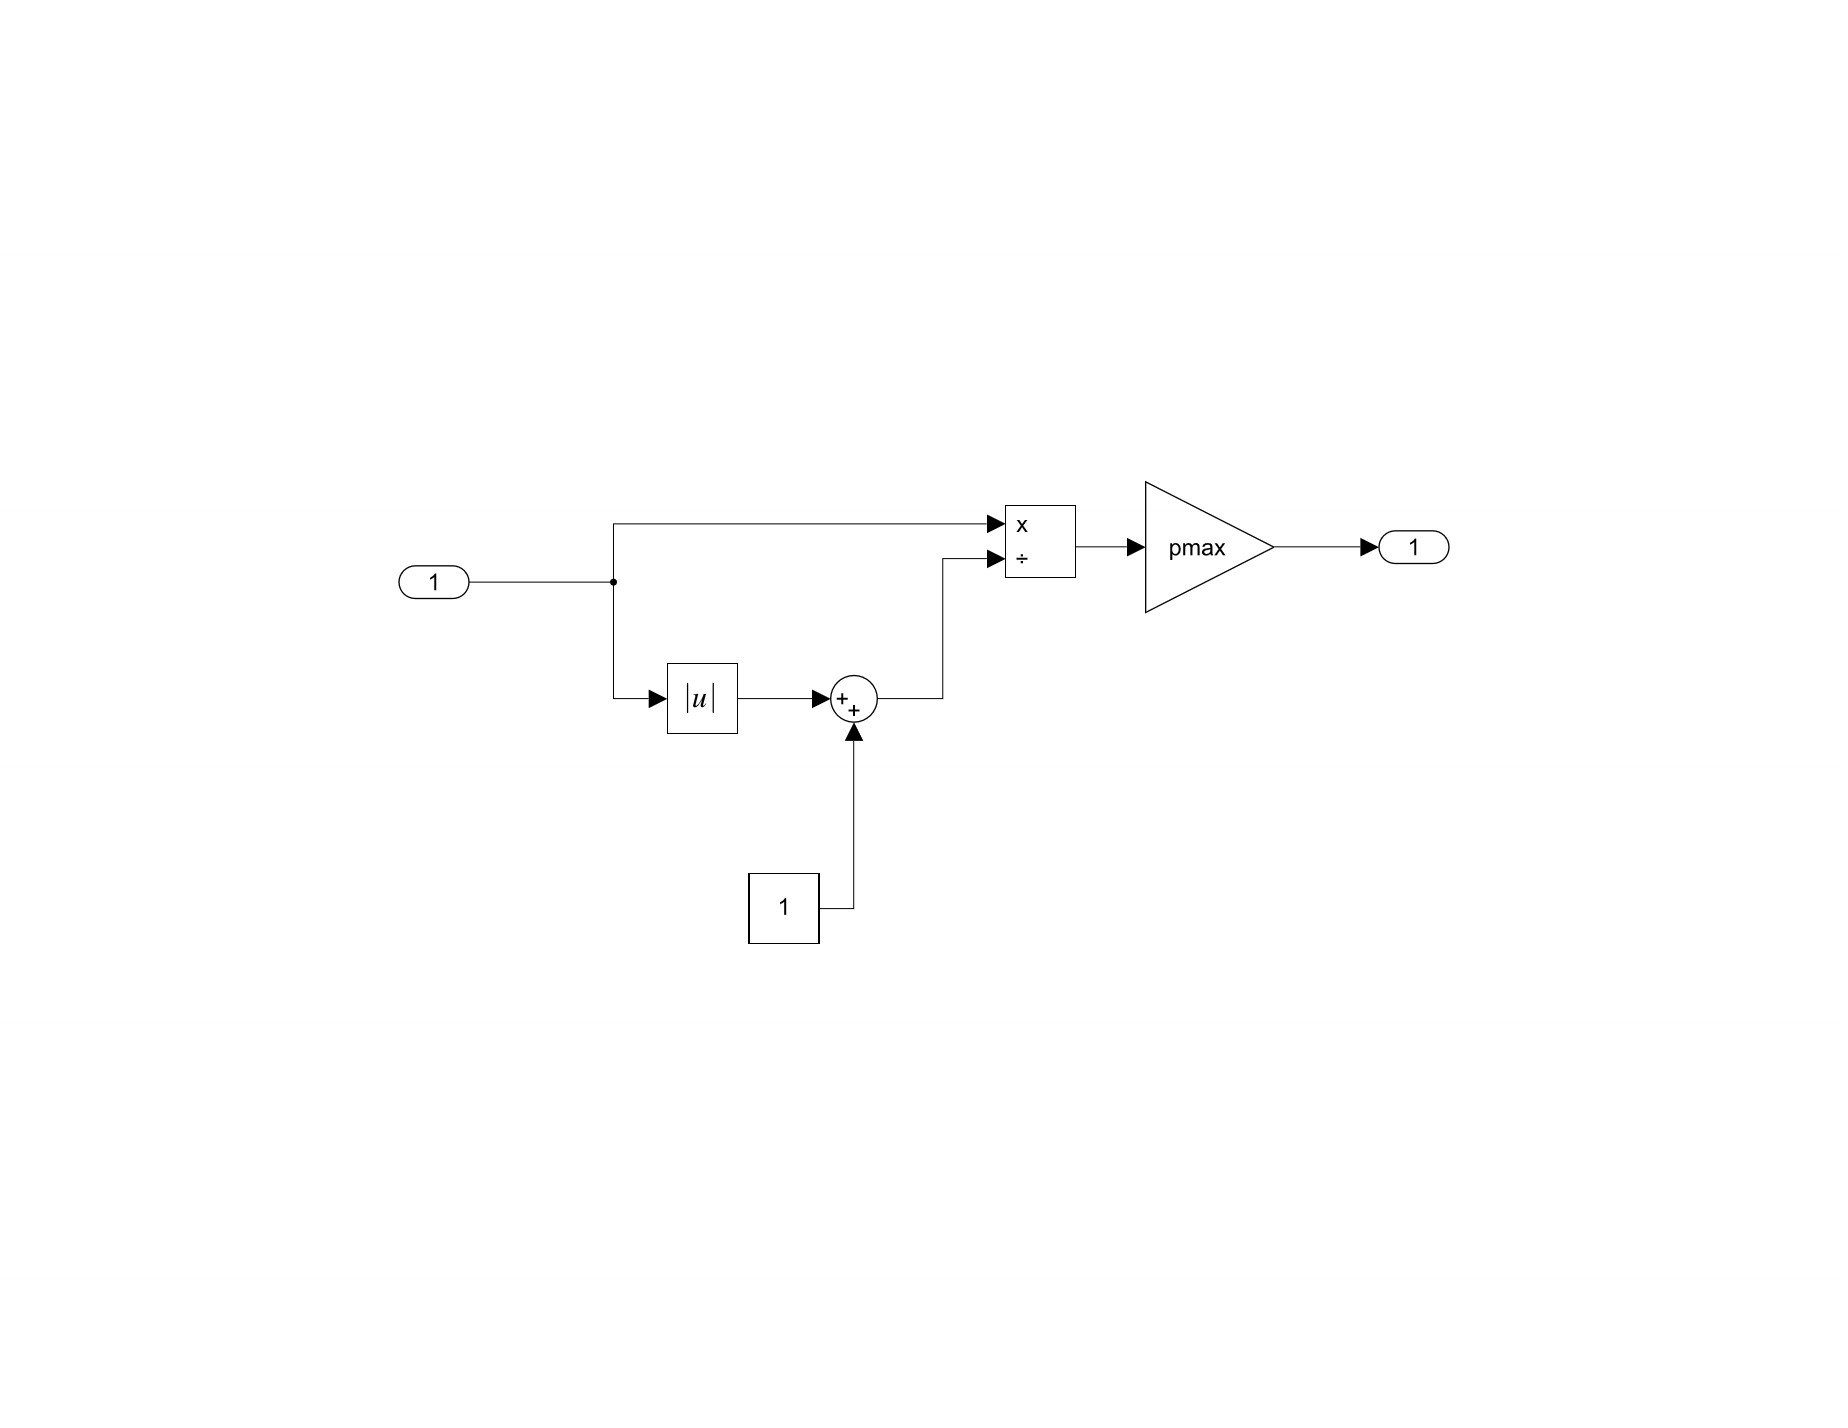
\includegraphics[width=\columnwidth]{/SimulinkModels/Controller/sigmoidal.jpg}%
	\end{center}
	\caption{Sigmoidal function Simulink subsystem.}%
\end{figure}

\begin{figure}[htb]
\begin{center}
	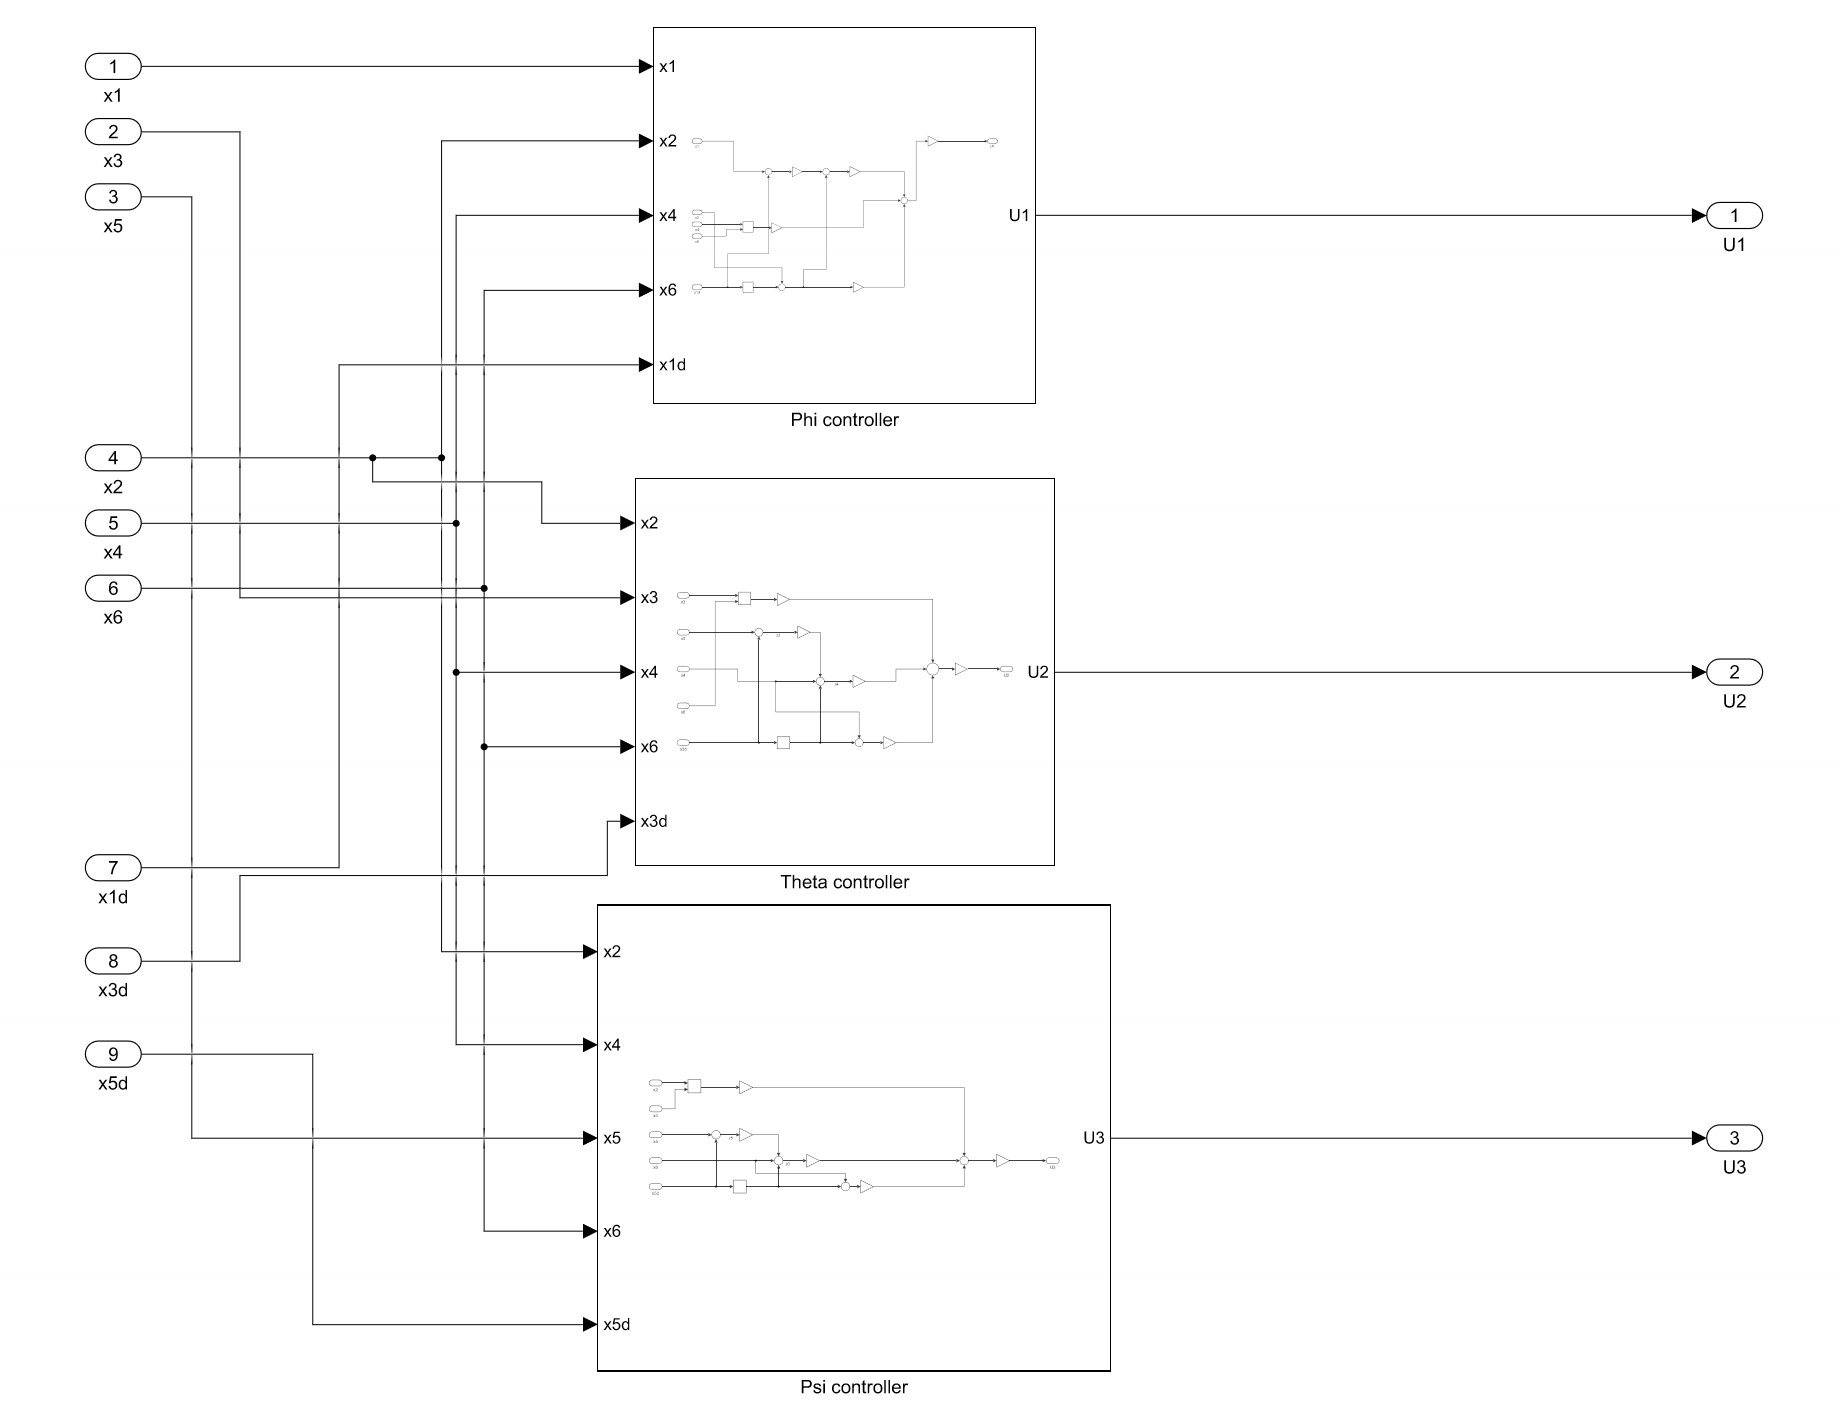
\includegraphics[width=\columnwidth]{/SimulinkModels/Controller/Angle.jpg}%
	\end{center}
	\caption{Angle controller Simulink subsystem.}%
\end{figure}

\begin{figure}[htb]
\begin{center}
	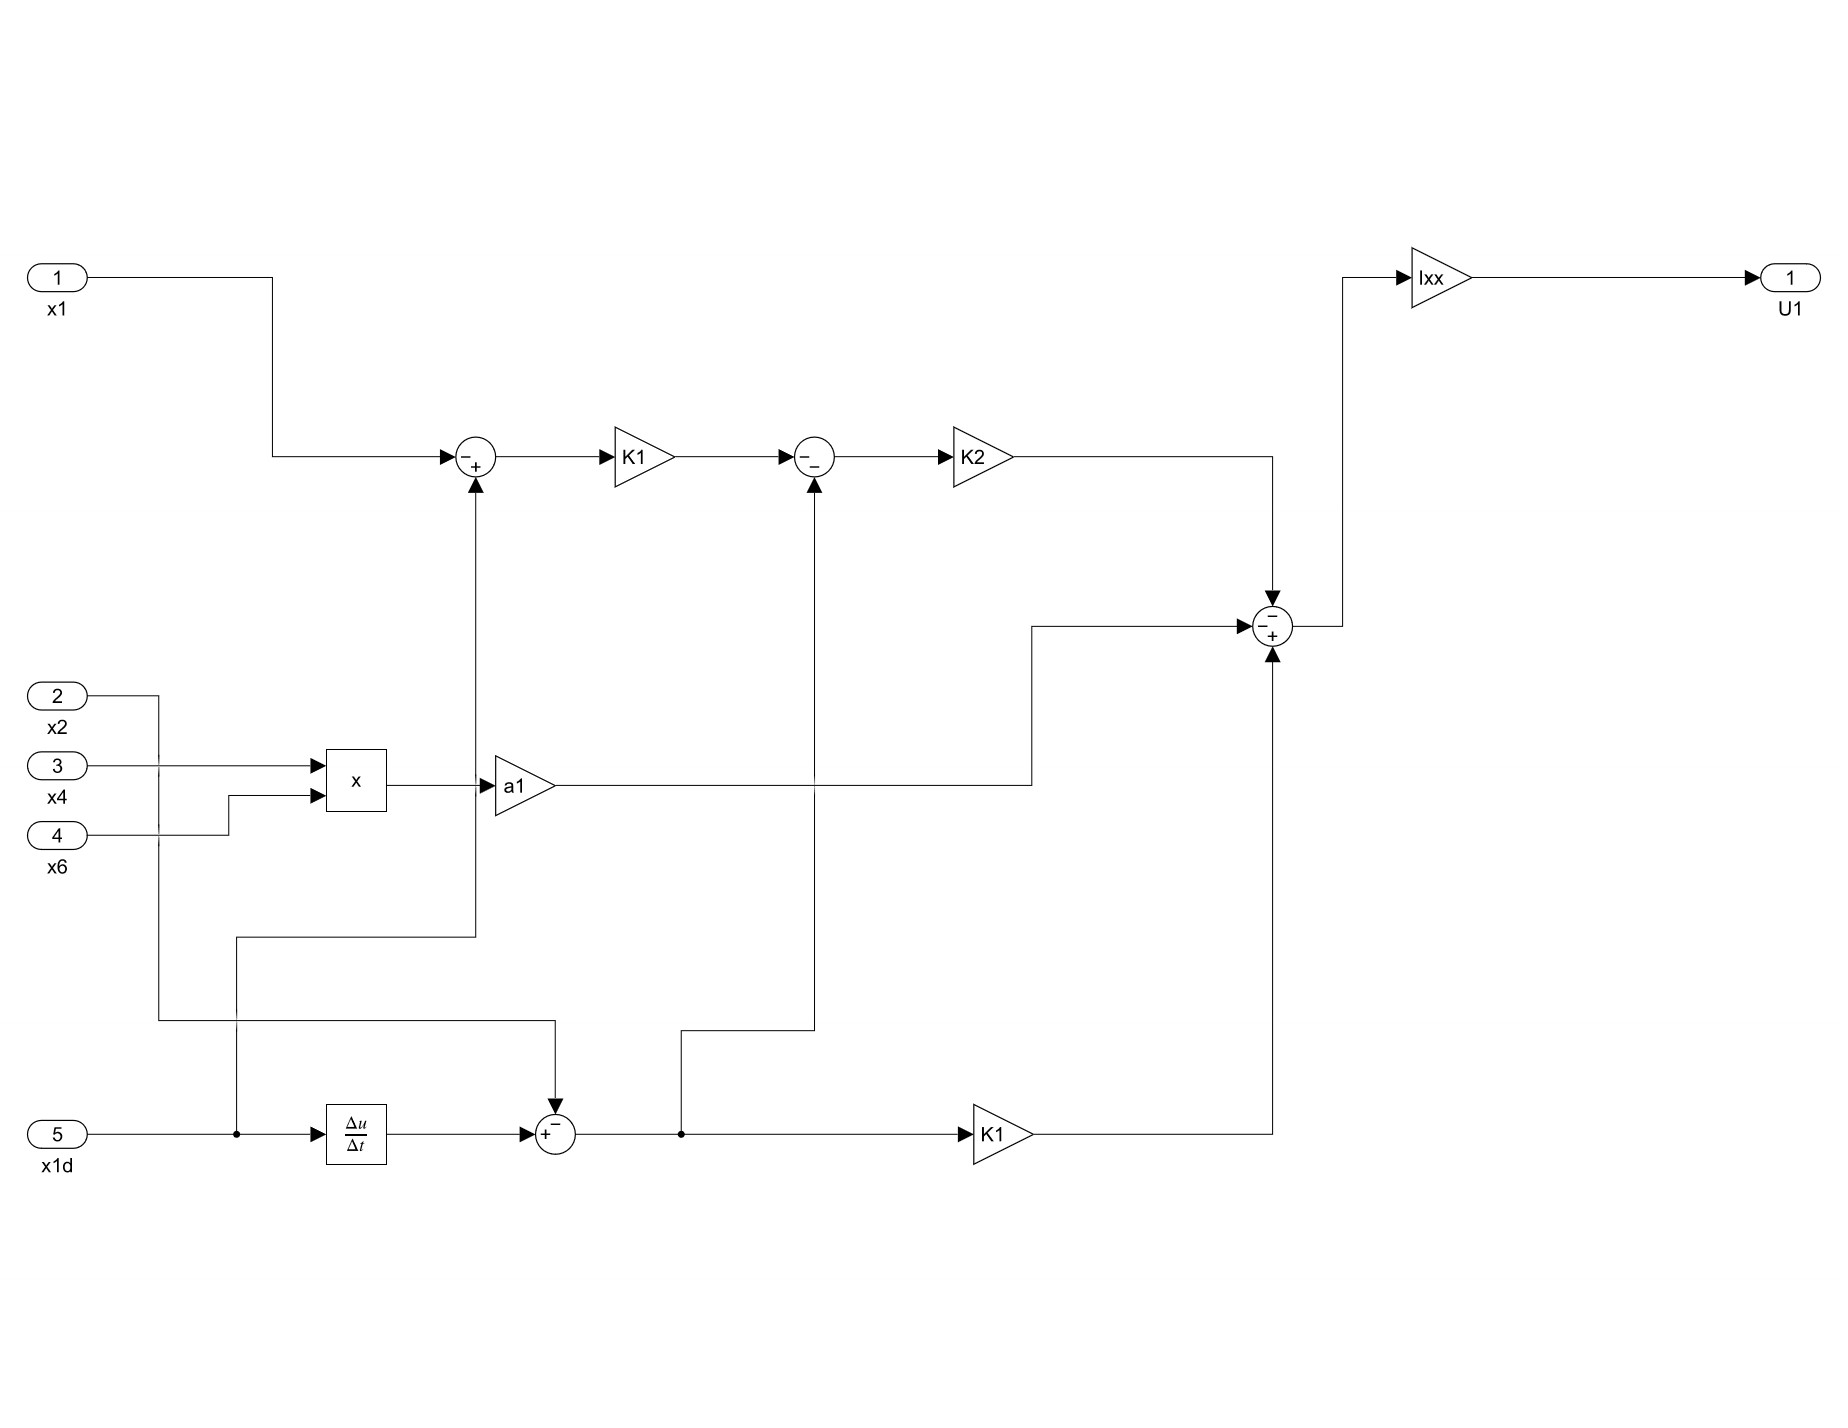
\includegraphics[width=\columnwidth]{/SimulinkModels/Controller/phi.jpg}%
	\end{center}
	\caption{Roll angle controller Simulink subsystem.}%
\end{figure}

\begin{figure}[htb]
\begin{center}
	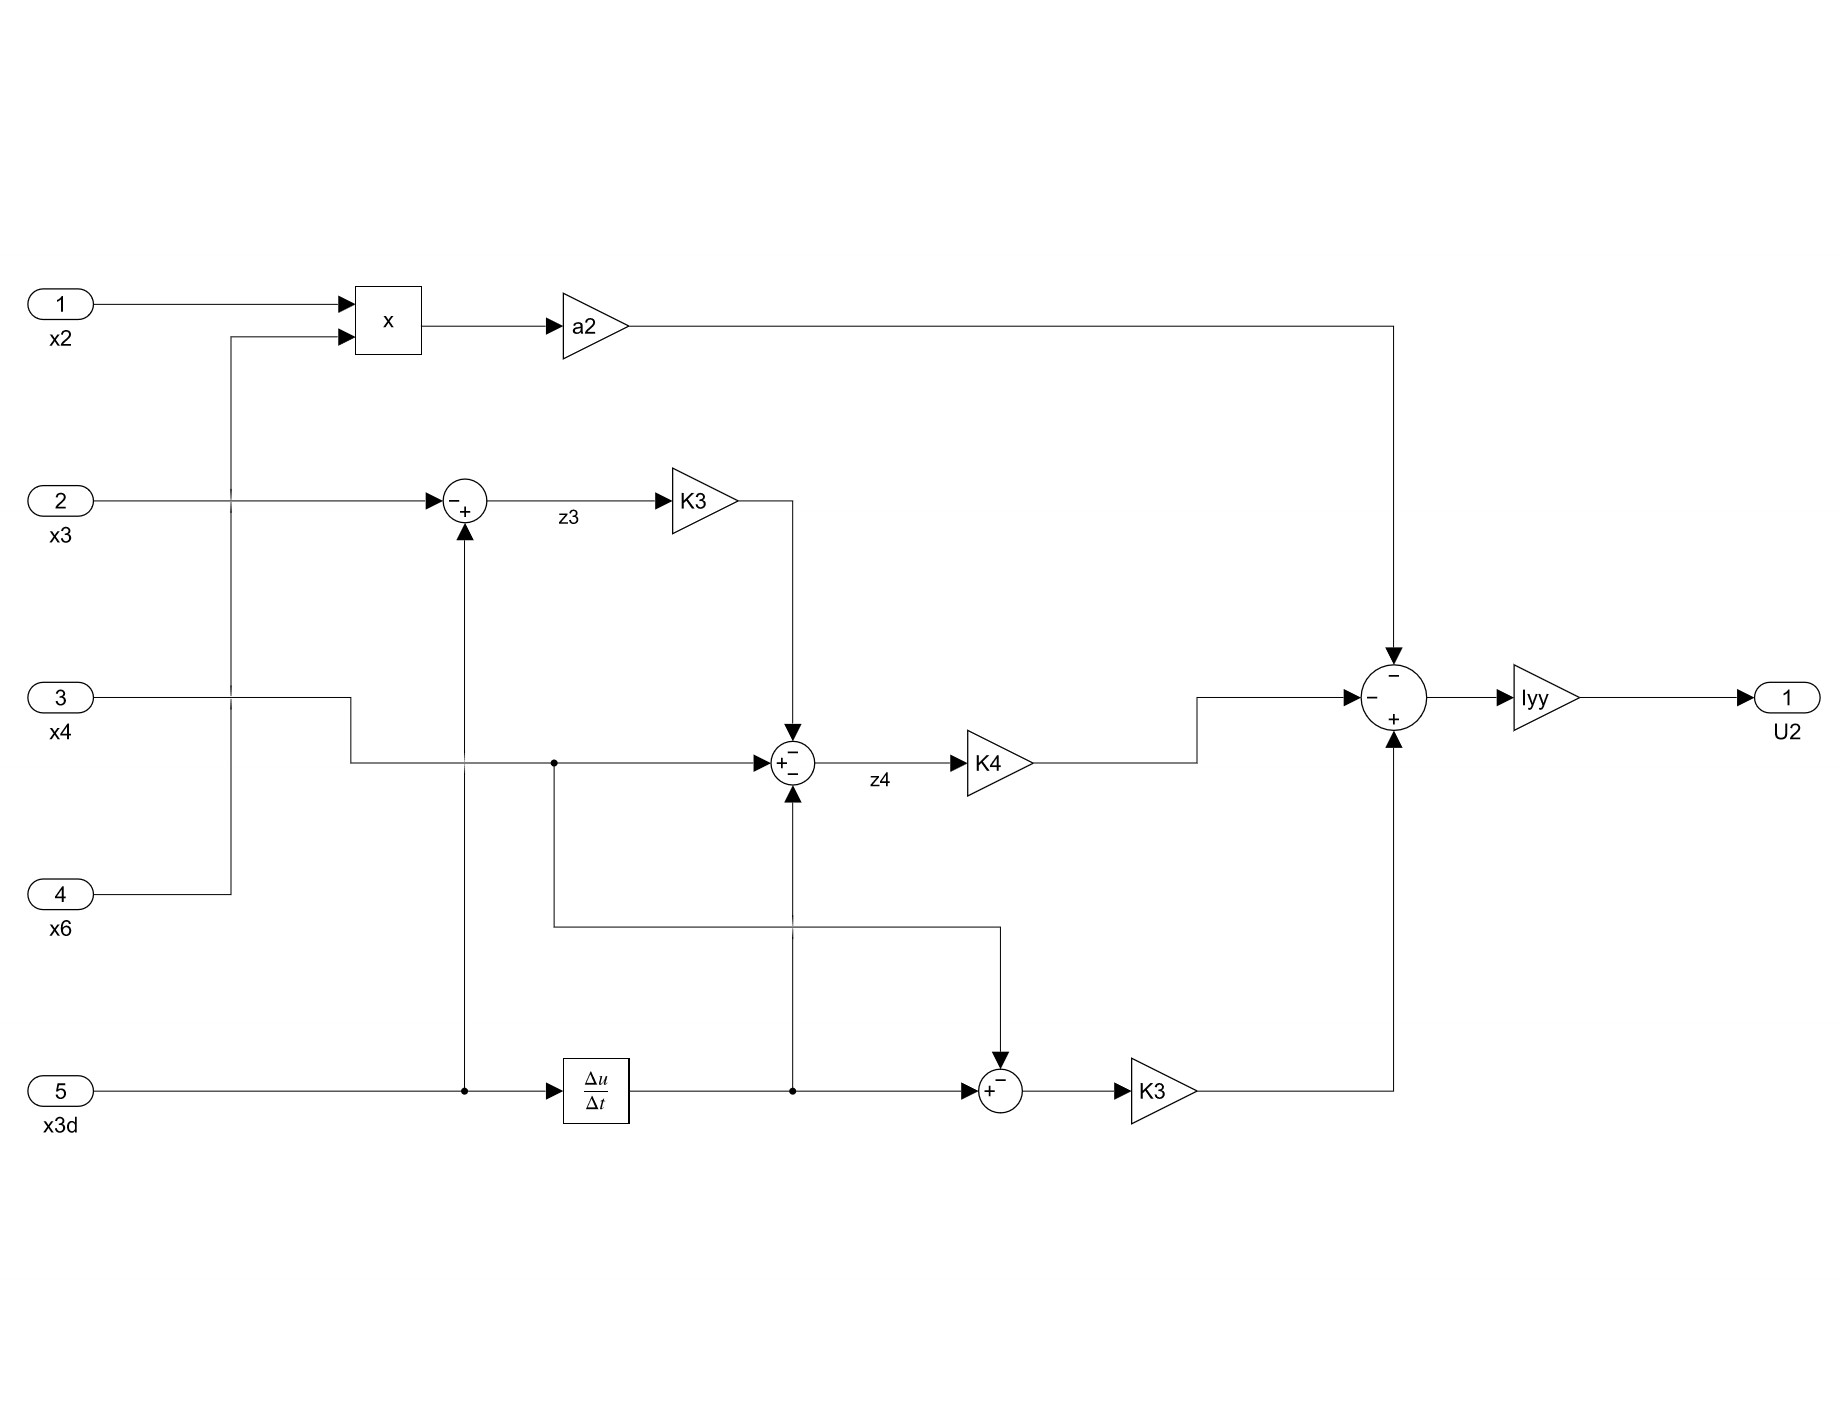
\includegraphics[width=\columnwidth]{/SimulinkModels/Controller/theta.jpg}%
	\end{center}
	\caption{Pitch angle controller Simulink subsystem.}%
\end{figure}

\begin{figure}[htb]
\begin{center}
	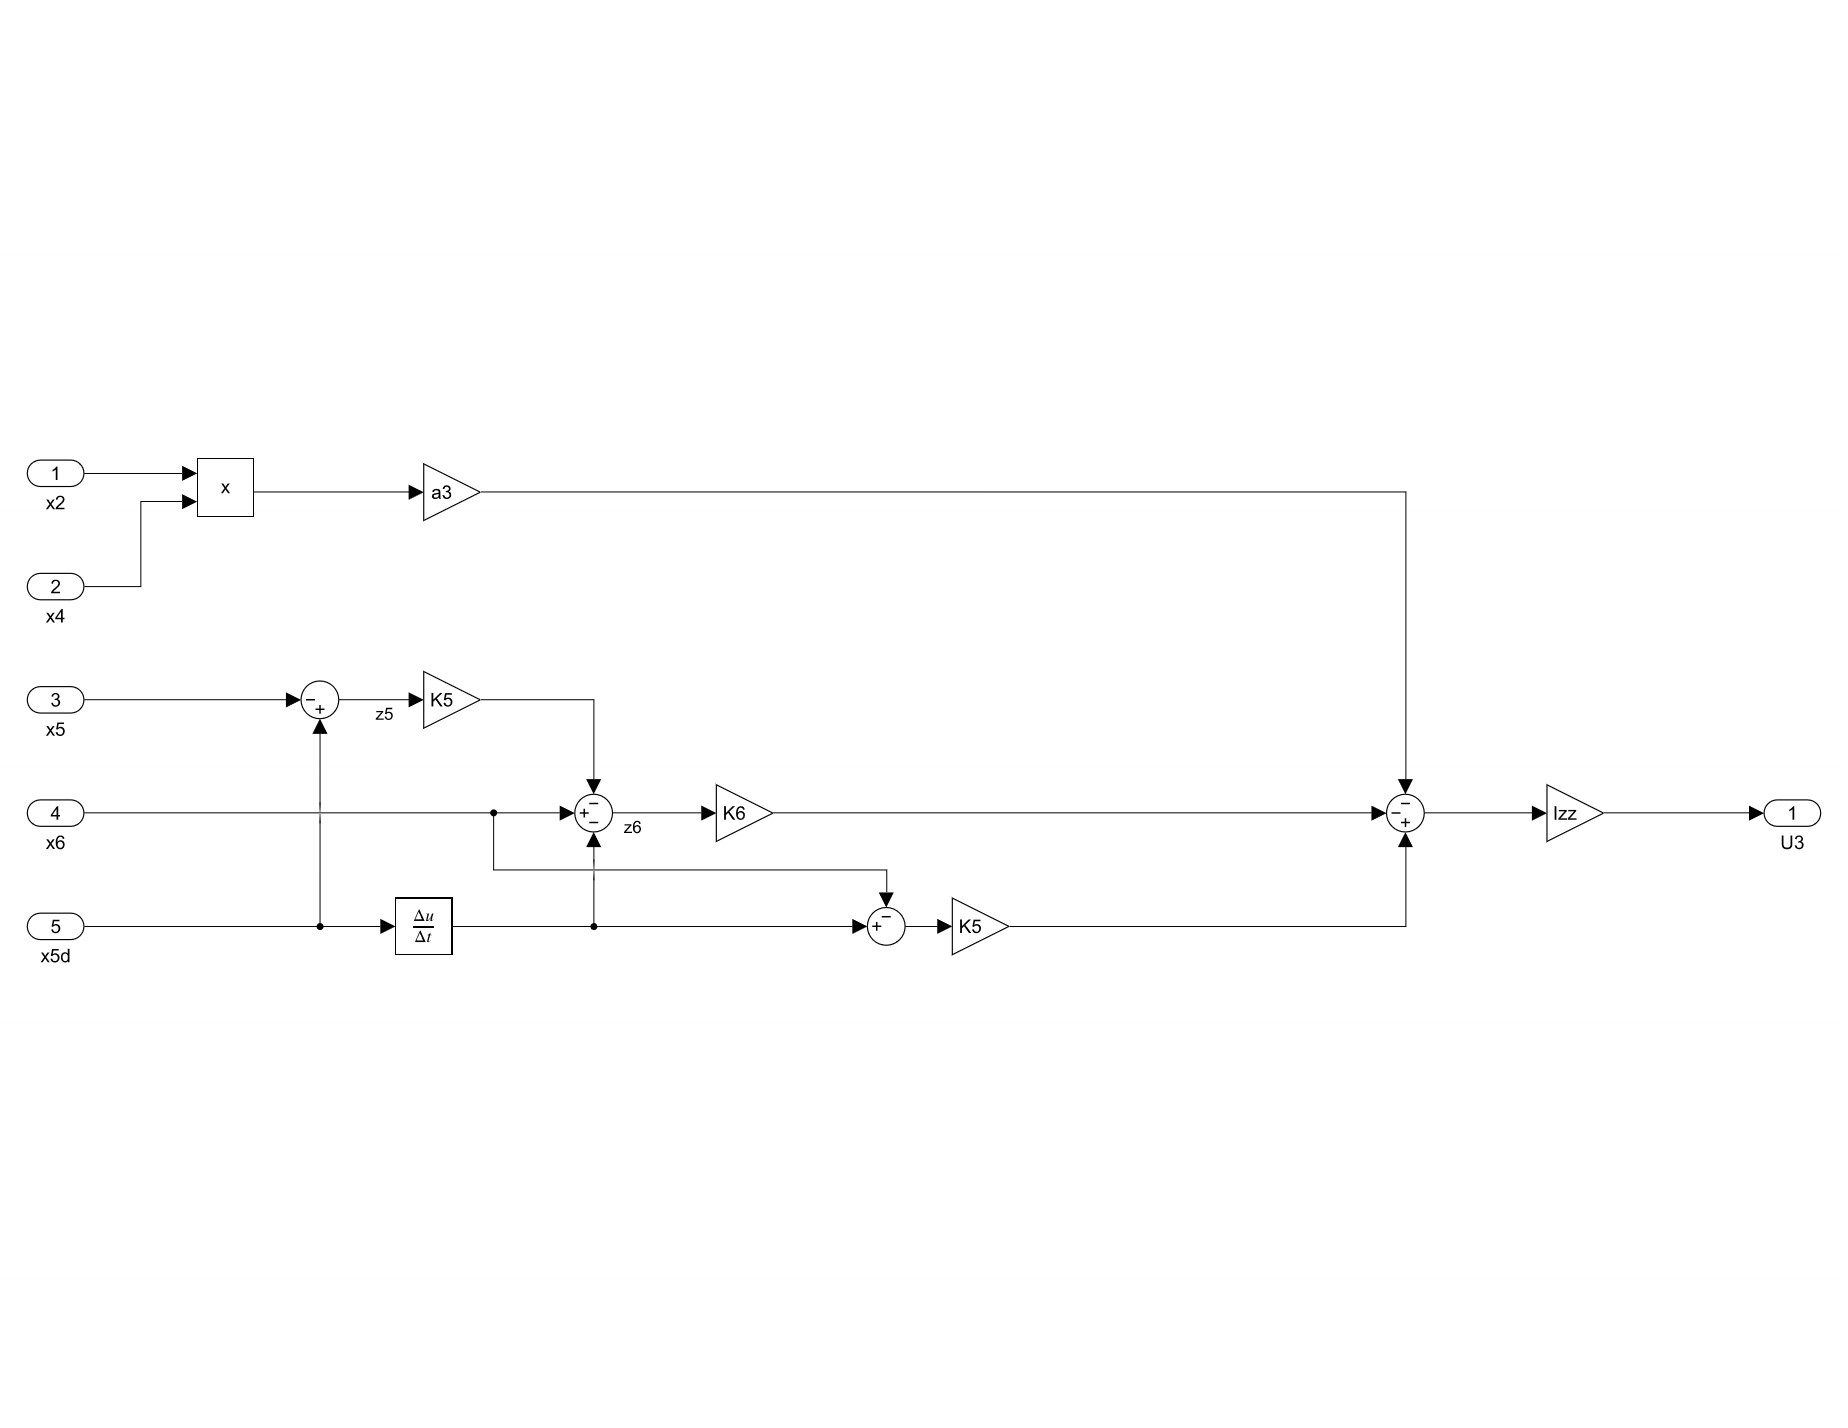
\includegraphics[width=\columnwidth]{/SimulinkModels/Controller/psi.jpg}%
	\end{center}
	\caption{Yaw angle controller Simulink subsystem.}%
\end{figure}

\clearpage